\documentclass[12pt]{article}
\usepackage[margin=1in]{geometry}
\usepackage{times}
\usepackage{graphicx}
\usepackage{float}
\usepackage{caption}
\usepackage{subcaption}
\usepackage{lineno}
\usepackage{amsmath}
\usepackage{multirow}
\usepackage{bm}
\usepackage{tabularx}
\usepackage{makecell}
\RequirePackage{booktabs}
%\usepackage{natbib,hyperref}
\linenumbers

\newcommand*{\met}{\ensuremath{E_\text{T}^\text{miss}} }
\newcommand*{\metvec}{\ensuremath{\vec{E}_\text{T}^\text{miss}} }
\newcommand*{\mindphi}{\ensuremath{\Delta \phi_{\text{jets}_{1,2,3} \met}} }
\newcommand*{\metnomu}{\ensuremath{E_\text{T}^{\text{miss}, \text{no} \mu}}}
\newcommand*{\ptll}{\ensuremath{p_{\text{T}}^{\ell \ell}}}

\author{\Large{Candidacy Report} \\
\\
Danika MacDonell}
\title{Search for Dark Matter Produced in Association with a Hypothetical Dark Higgs Boson Decaying to $W^+W^-$ in the $q\bar{q}\ell\nu$ Final State Using $pp$ Collisions Recorded with the ATLAS Detector}
\begin{document}
\maketitle

\section{Introduction}

The proposed thesis is a search for dark matter (DM) using high energy proton-proton ($pp$) collision data recorded with the ATLAS detector at the Large Hadron Collider (LHC). The search targets a final state signature of DM production in association with the emission of a hypothetical higgs boson $s$ in the dark sector, which subsequently decays to a pair of W bosons. The search is motivated by and optimized with a ``dark higgs model" \cite{dark_higgs} shown in figure \ref{fig:signal_model}, in which the $s$ is emitted from a hypothetical $Z'$ gauge boson in the dark sector, which itself mediates the production of DM particles from the annihilation of ``initial state quarks" (IS $qq$) constituting the colliding protons.  

\begin{figure}[H]
	\centering
	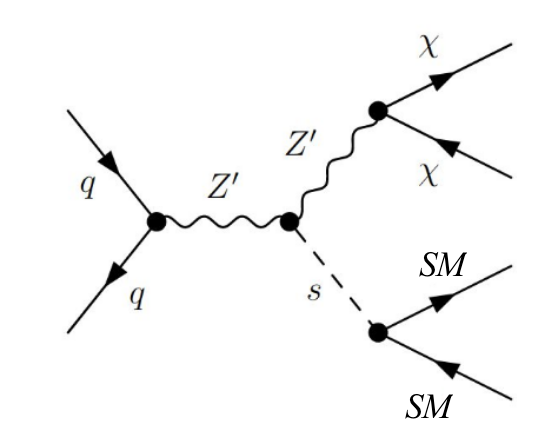
\includegraphics[width=0.4\textwidth]{figures/Signal_generic.png}
	\caption[]{Dark higgs model}
	\label{fig:signal_model}
\end{figure}

Any DM that may be produced in the $qq$ collisions is expected not to interact to any measurable extent with the `normal' matter constituting the detector. As such, it is assumed that the momentum carried by the DM would escape the detector undetected. The law of momentum conservation, which requires the vector sum of momenta of all measured particles produced by the collision to match that of the initial state quarks, can be used to infer the presence of undetected particles if the IS quark momenta are known. As the fraction of proton momentum carried by each of the IS quarks - described by ``parton distribution functions" (PDFs) \cite{PDF_Review} - is statistical in nature, their momenta in the direction of the $pp$ beam line cannot be known precisely. However, IS quark momentum in the plane transverse to the beam line is in general negligibly small compared with the collision energy, so it can be expected to a high degree of precision that the final state particle momenta in this transverse plane will sum to zero. This expectation implies that DM produced at the LHC will exhibit a signature of high missing transverse momentum in the final state. This two dimensional missing transverse momentum vector is typically denoted ``\metvec", and its magnitude ``\met":

\begin{equation}
\metvec = -\sum_i \vec{p}_{x, i} + \vec{p}_{y, i}
\end{equation}

\noindent where the sum is over all visible particles in the event.

The aim of the proposed thesis work is to apply selections, including a requirement of high \met, to data from the ATLAS detector to optimize the sensitivity of the data to the dark higgs signal model. The data will subsequently be compared with standard model (SM) background and signal processes simulated with Monte Carlo to search for an above-background excess in the data consistent with the signal model. 

The search is split into two separate analyses:

\begin{enumerate}

\item \textbf{The hadronic decay channel:} In this channel, each of the two W bosons in the final state decay to quarks, which subsequently hadronize in the detector and are measured as jets in the ATLAS calorimeter.

\begin{equation}
\nonumber
WW \rightarrow q\bar{q}+q\bar{q}
\end{equation}

Given that the branching fraction for hadronic W decay is 0.68 \cite{PDG}, the fully hadronic WW decay occurs with a branching fraction of 0.46 ($=0.68^2$). In addition to its substantial branching fraction, this channel has the advantage of being able to fully reconstruct the momenta of both W bosons, and as such the $s$ mass. The drawback is that there are SM processes with large production cross section which also produce a final state of multiple jets in the detector, a subset of which pass the other signal selection criteria and represent a sizeable background in the analysis. 

\item \textbf{The semileptonic decay channel:} One W boson decays to quarks in this channel, and the other decays to a lepton and a neutrino, where the lepton $\ell$ is either an electron or a muon. 

\begin{equation}
\nonumber
WW \rightarrow q\bar{q}+\ell\nu
\end{equation}

Despite its lower branching fraction of 0.29 \cite{PDG} compared with the fully hadronic decay channel, the semileptonic channel has the advantage that the requirement of having one lepton in the final state reduces the background of SM processes. However, this comes at the cost of additional \met from the neutrino production, which both inhibits full reconstruction of the leptonically-decaying W boson and cannot easily be distinguished from the \met associated with DM production in the signal model. 

\end{enumerate}

There is a mature analysis searching for the dark higgs signal in the hadronic decay channel, and the proposed thesis will focus on the semileptonic decay channel. 

The WW decay can also proceed via a fully leptonic channel, in which both W bosons decay to a lepton and a neutrino. This channel would give a clean signature of two leptons and no jets, but is currently not considered as a viable search channel due to its relatively low branching fraction of 0.046 \cite{PDG}.

Once the analysis is fully developed in the semileptonic decay channel, this channel will be statistically combined with the hadronic search channel. In the event that the combined search does not show an above-background excess, the analysis will place exclusion limits - at some specified level of confidence, typically 95\% - on the range of $Z'$ and $s$ masses in the dark higgs model to which the combined search is sensitive.

\section{Motivation}

The proposed thesis work would contribute to the extensive ongoing DM search program at the LHC. The LHC search program is motivated by compelling evidence from observational astronomy for the existence of DM constituting 85\% \cite{planck} of all matter in the universe. Despite clear evidence from observational astronomy for its gravitational interactions with normal matter, DM has yet to be detected through the weak, strong or electromagnetic interactions. As such, its composition and non-gravitational interactions - if any - remain largely a mystery. The current most widely accepted and theoretically motivated DM candidates take the form of fundamental particles, yet there is no particle in the standard model of particle physics that could represent a viable DM candidate \cite{feng}. DM is therefore widely assumed to be a ``beyond-standard-model" (BSM) particle. 

\subsection{Dark Matter Search Methods}
There are three complementary approaches used to search for particle DM: direct and indirect detection, and collider searches. Direct detection searches \cite{Schumann_2019, 2015gya} aim to directly detect evidence of a recoil induced by elastic scattering between a DM particle in the galactic halo passing through the detector and a target particle in the detector. Indirect searches \cite{CIRELLI_2012, conrad} use observational data to search for evidence of products produced by DM annihilation or decay in particular regions of the observable universe expected to have a high DM density. Collider searches \cite{DM_colliders}, of which the proposed thesis work is an example, study the decay products from high-energy collisions of subatomic particles to search for an above-background excess of events that could be consistent with DM having been produced in some of the collisions.

\subsection{Models of Dark Matter Production at Colliders}
Models of DM production in colliders can range in complexity from an effective field theory (EFT), where the DM production mechanism is completely unspecified, to a complete model such as supersymmetry \cite{susy_dm}, which predicts viable DM candidates as part of a hypothesized extension to the SM designed to address a range of phenomena unexplained by the SM. 

%The EFT approach treats the production of DM from colliding partons as a contact interaction, with the production rate determined by a single parameter \cite{DM_colliders}. As long as a measurable SM particle is also produced in the interaction (eg. a gluon radiating from one of the colliding quarks, see figure \ref{fig:eft_simplified_model}), the EFT framework can be applied to any mono-X signature at the LHC, where a SM particle X is measured along with missing transverse momentum in the detector. This makes the framework generally usable in terms of motivating and providing a theoretical framework to interpret a range of generic search channels that can be readily selected for in LHC collision data. However, the EFT framework relies on the assumption that the the mediator(s) of the interaction is (are) much more massive than the scale of momentum transfer in the interaction \cite{DM_colliders, beyond_eft}. If this assumption is inaccurate, the EFT framework becomes invalid, and a more complete model is needed to specify additional details of the process leading to DM pair production. 

\begin{figure}[H]
	\centering
	\begin{minipage}[b]{0.45\textwidth}
	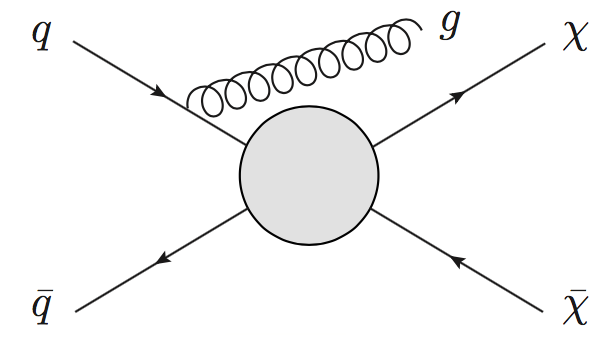
\includegraphics[width=0.9\textwidth]{figures/EFT_Signature.png}
	\end{minipage}
	\begin{minipage}[b]{0.45\textwidth}
	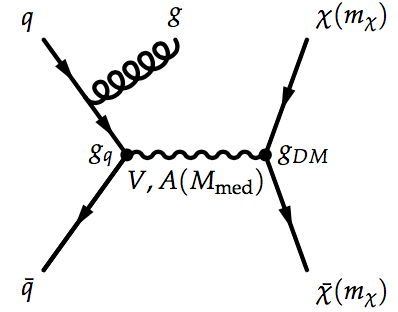
\includegraphics[width=0.8\textwidth]{figures/simplified_model.png}
	\end{minipage}
	\caption[]{Left: Mono-jet process in the EFT framework (source: \cite{beyond_eft}). Right: Mono-jet process in a simplified model framework, where the pair production of DM occurs via a new vector or axial-vector ($V$, $A$) mediator of mass $M_\text{med}$, which couples to quarks and DM with coupling constants g$_q$ and g$_\text{DM}$, respectively (source: \cite{dm_forum})}.
	\label{fig:eft_simplified_model}
\end{figure}

In principle, complete theories of physics beyond the SM, such as the minimal supersymmetric SM (MSSM) \cite{mssm} can offer theoretically motivated and experimentally accessible models which specify the details of candidate processes by which the colliding partons may annihilate to produce DM. However, these theories tend to be quite complex, with many free parameters - over 100 in the case of MSSM \cite{DM_colliders} - most of which need to be fixed to generate a reasonably testable model. Relying on complete theories alone to guide experimental signatures may run the risk of missing important parameter space of new physics for which a complete theory has not yet been developed. 

Simplified models, widely used in recent and ongoing DM searches at the LHC, are designed to bridge the gap between EFT and complete theories. They provide a `first-order' description of theoretically motivated new physics scenarios that could be accessible at collider energies. They provide guidance for experimental searches without fully specifying the details of any additional new physics at energies above the collider scale that would be needed for a complete theory \cite{DM_colliders}. In terms of DM production at the LHC, one or more new mediators associated with new physics scenarios may be considered which allow for mixing between SM particles and DM. The process by which the mixing occurs is represented with a tree-level diagram whose experimental signature would be accessible at LHC energies, such as the diagram shown in figure \ref{fig:eft_simplified_model} which represents a DM benchmark model featured in the 2015 report of the ATLAS/CMS Dark Matter Forum \cite{dm_forum}.

\subsection{Dark Higgs Model}

The proposed search is motivated by and interpreted with a simplified model described in \cite{dark_higgs} where DM is pair produced from a Z boson in the dark sector - known as the $Z'$ boson - in association with the emission of a dark sector higgs boson $s$. Figure \ref{fig:signal_model} shows one of the leading order Feynman diagram representing this simplified model. The dark sector higgs boson subsequently decays to a pair of massive SM particles through a small mixing with the SM higgs boson. 

The generic hypothesis of `dark sector' mediators which exhibit a small mixing with SM particles is motivated in part by the theoretical need for creation and annihilation mechanisms between DM and SM particles in the well-motivated and popular `thermal freeze-out' hypothesis \cite{particle_dm}. In the thermal freeze-out hypothesis, DM and SM particles interacted at a sufficient rate in the high temperature and matter density of the early universe to remain in thermal equilibrium. Once the DM-SM interaction rate dropped below the expansion rate of the universe, the DM rapidly ``froze out" of thermal equilibrium with the SM particles, at which point the relic abundance of DM was fixed to the value observed in the present-day universe.

The dark higgs boson in particular is motivated by the need to generate the masses of DM and any other particles residing in the dark sector \cite{dark_higgs}. If dark sector particle masses are generated via a `dark sector higgs mechanism', this would naturally imply the existence of a dark higgs boson. 

The model presented in \cite{dark_higgs} considers a scenario in which there is another dark sector mediator - taken to be the $Z'$ - with a mass within the range accessible to measurement at the LHC, which mediates DM production from parton collisions. In this case, the $Z'$ could radiate a dark higgs boson. Theoretically, the observed relic abundance of DM in the universe suggests that couplings between particles in the dark sector should be quite large, which could result in a sufficiently high probability of dark higgs emission from the $Z'$ to produce a measurable signature in LHC collisions \cite{dark_higgs}. 

Experimentally, the dark higgs signature would be distinct from generic mono-X signatures where the SM particle that the DM recoils against is produced via initial state radiation (as shown in figure \ref{fig:eft_simplified_model}, because as long as the mass of the $s$ is well below the typical momentum transfer of the collisions, the $s$ will tend to be highly boosted in the plane transverse to the beam line. As a result, the SM decay products will tend to be much higher in transverse momentum and highly collimated compared with particles produced via initial state radiation.  

\subsection{Experimental Background}

This section discusses a previous experimental search which set exclusion limits on the dark higgs model described in Section 2.3, in the case where the dark higgs decays to a pair of b quarks. It goes on to describe the m$_\text{S}$ range that the ongoing and proposed searches in the $s \rightarrow WW$ decay channel target, and explain how this target is complementary to the m$_\text{S}$ range explored by the previous search in the $s \rightarrow bb$ channel. 

\subsubsection{Re-interpretation of Mono-H(bb) Search with a Dark Higgs Mediator}

Last year, the ``mono-H(bb)" DM search, originally published in 2018 \cite{monohbb} with 79.8 fb$^{-1}$ of data taken with the ATLAS detector at a 13 TeV centre of mass energy, was re-interpreted \cite{monohbb_recast} using the RECAST framework \cite{recast} to set exclusion limits on the dark higgs model in the case of the dark higgs decaying to a pair of b-quarks. 

The mono-H(bb) search selects for a final state of missing transverse energy along with two jets in the calorimeter, both of which must be tagged as having originated from the hadronization of b quarks. When the mono-H(bb) analysis was originally published, it had been developed and interpreted using a simplified model shown in figure \ref{fig:monohbbreinterp} left, in which the DM is pair produced from a new pseudoscalar higgs boson, along with the emission of a SM higgs boson, which subsequently decays to two b quarks.  

The original analysis was preserved using RECAST \cite{recast}, a framework designed to preserve searches for new physics with high energy collision data in such a way that the searches can be readily re-analyzed with alternative models of new physics which predict the same final state signature. The RECAST framework was used to re-interpret the mono-H(bb) search using the dark higgs model shown in figure \ref{fig:monohbbreinterp} right, where the dark higgs, whose mass is left as a floating parameter, decays to a pair of b quarks. 

\begin{figure}[H]
	\centering
	\begin{minipage}[b]{0.45\textwidth}
	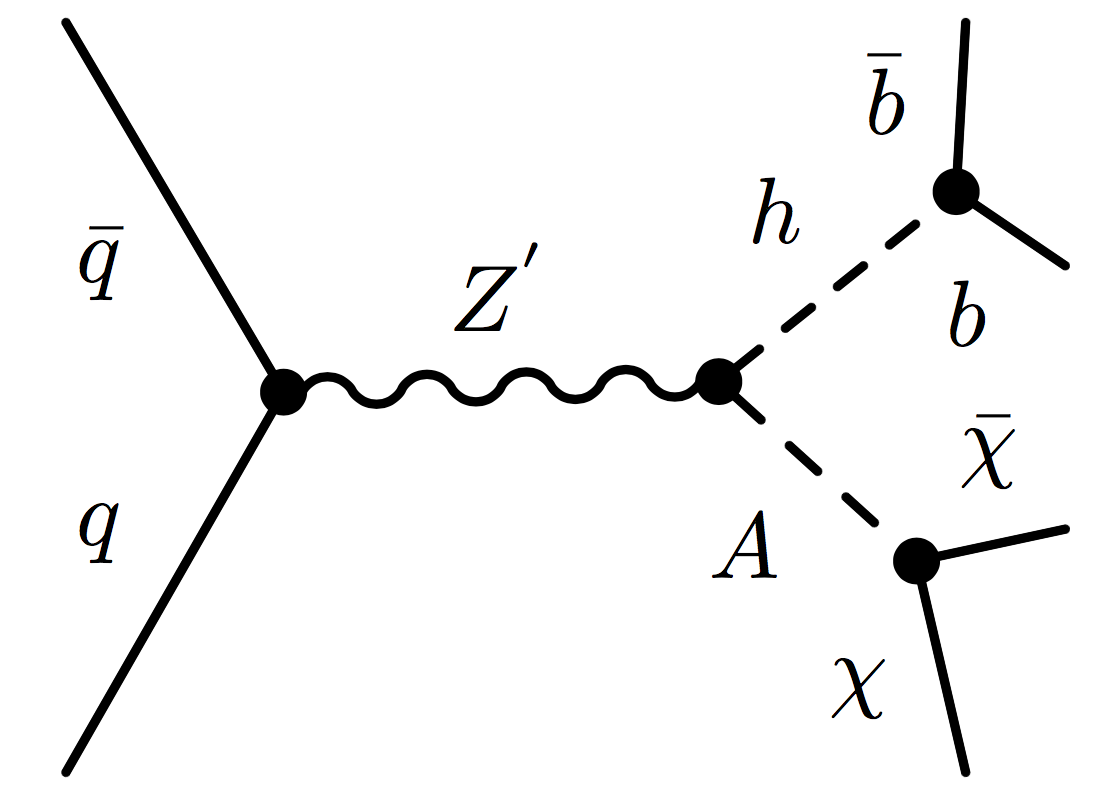
\includegraphics[width=0.8\textwidth]{figures/monohbb}
	\end{minipage}
	\begin{minipage}[b]{0.45\textwidth}
	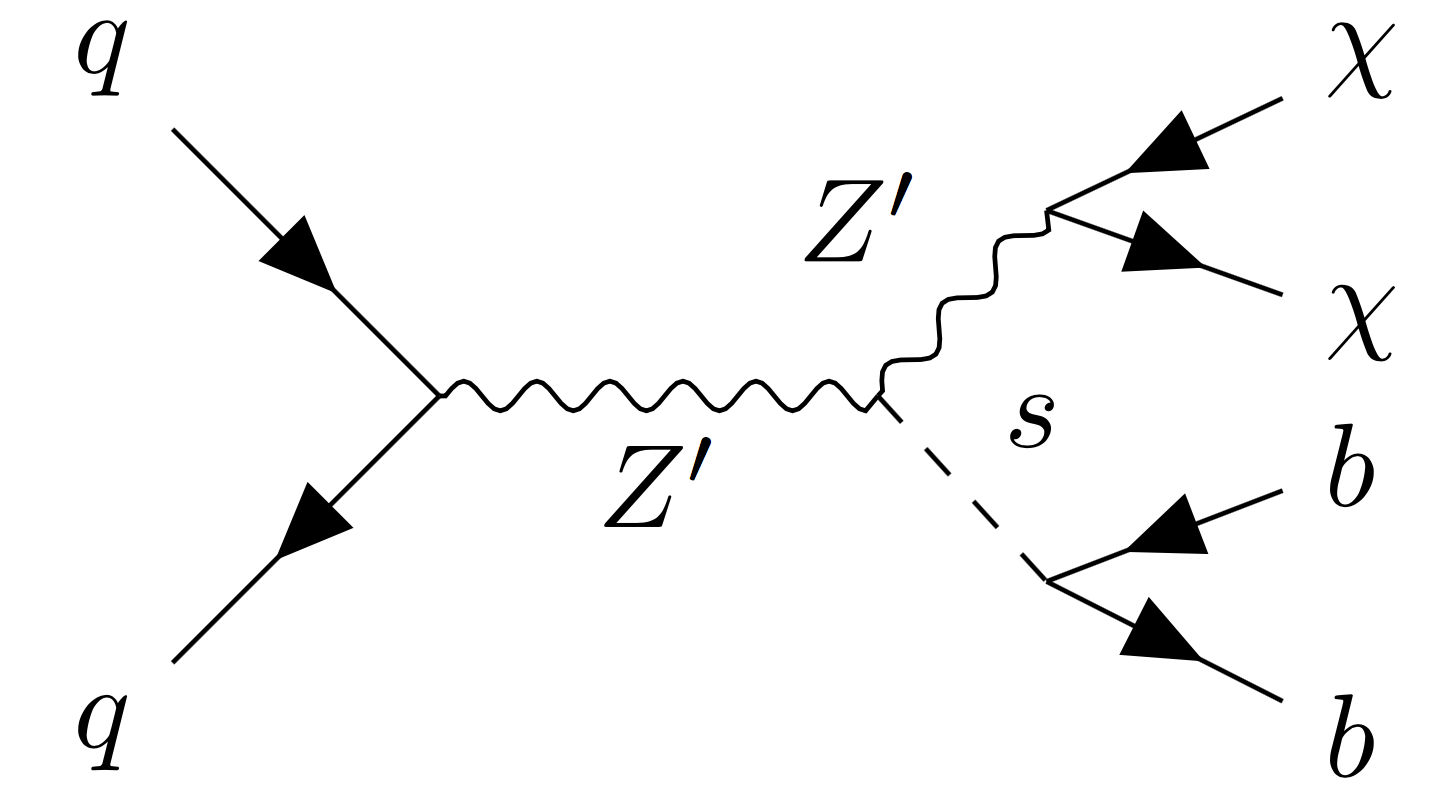
\includegraphics[width=0.9\textwidth]{figures/monosbb}
	\end{minipage}
	\caption[]{Left: Leading-order Feynman diagram representing the model used to interpret the mono-H(bb) DM search. Right: A leading-order Feynam diagram representing the model used to guide and interpret the mono-s(bb) re-interpretation of the mono-H(bb) search. The dark higgs mediator mass m$_\text{S}$ is allowed to float in the dark higgs model.}
	\label{fig:monohbbreinterp}
\end{figure}

The re-interpreted mono-H(bb) search set limits, shown in figure \ref{fig:monosbb_exclusion}, on the phase space of $Z'$ and $s$ masses excluded by the data. To set these exclusion limits, several free parameters in the dark higgs model need to be fixed, as detailed in Section 6.1.1.
%
%\begin{itemize}
%\item The DM mass m$_\chi$ is fixed to 200 GeV.
%\item The constant g$_q$ associated with the coupling of the $Z'$ boson to quarks is fixed to 0.25.
%\item The constant g$_\chi$ associated with the coupling of the $Z'$ boson to DM is fixed to 1.0.
%\item The mixing angle $\theta$ between the dark and SM higgs bosons is fixed to 0.01.
%\end{itemize}

\begin{figure}[H]
	\centering
	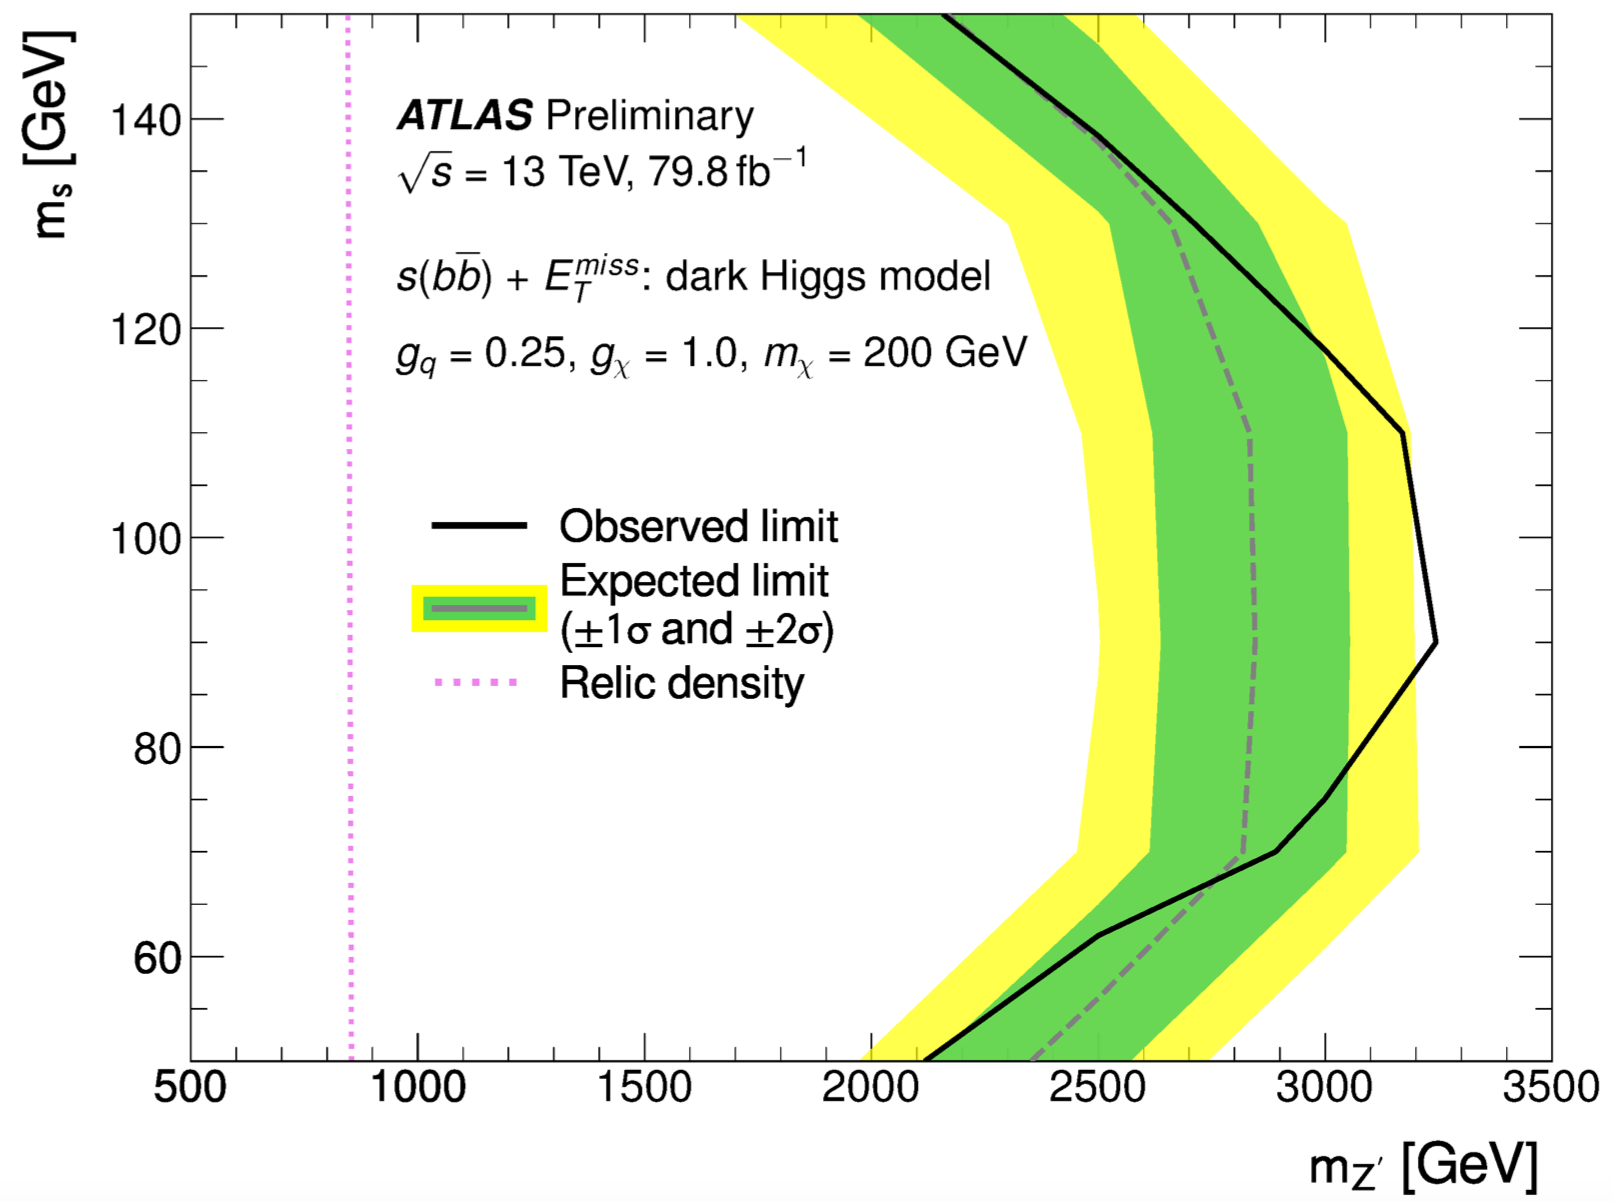
\includegraphics[width=0.7\textwidth]{figures/monosbb_exclusion.png}
	\caption[]{Exclusion limits set on the $Z'$ and $s$ mediator masses by the mono-H(bb) search re-interpreted with the dark higgs model. Mass combinations to the left of the solid black curve are excluded at a 95\% confidence level. Source: \cite{monohbb_recast}}
	\label{fig:monosbb_exclusion}
\end{figure}

%The values of $g_q$ and $g_\chi$ were chosen to match the conventional choices used by other LHC DM searches, and $\theta$ matches the choice used in the original paper \cite{dark_higgs} that introduced the dark higgs model.

\subsubsection{Dark Higgs Decay Modes}

The re-interpreted mono-H(bb) search probed the dark higgs model in the case where the $s$ emitted from the $Z'$ mediator decays to a pair of b quarks. However, predictions of the dark higgs branching ratio presented in the re-interpretation paper \cite{monohbb_recast} and shown in figure \ref{fig:higgsbrs} indicate that the $s \rightarrow bb$ decay mode is only sensitive to a range of dark higgs masses up to $\sim$150 GeV, above which the WW decay mode dominates in sensitivity. 

\begin{figure}[H]
	\centering
	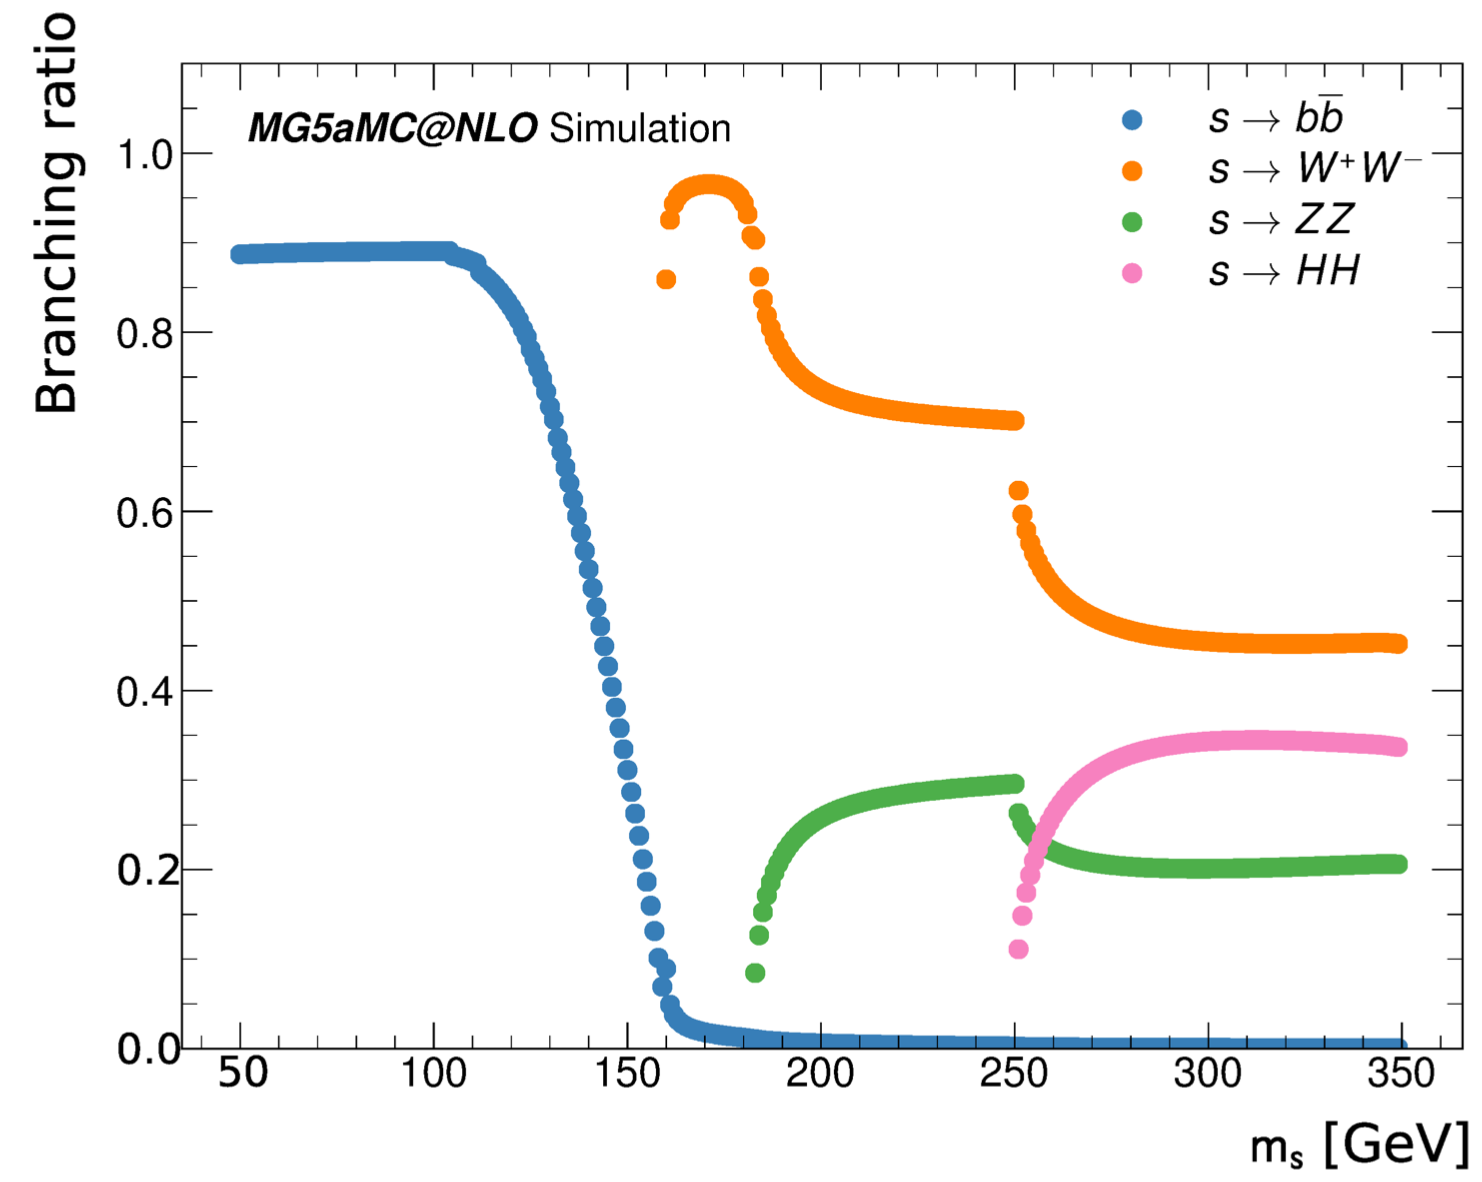
\includegraphics[width=0.7\textwidth]{figures/BR_vs_mass.png}
	\caption[]{Predicted dark higgs decay branching ratios as a function of dark higgs mass. Source: \cite{monohbb_recast} }
	\label{fig:higgsbrs}
\end{figure}

There is no a-priori reason to expect the dark higgs mass m$_\text{S}$ to necessarily lie below 150 GeV. Therefore, it's important to probe the model in the higher m$_\text{S}$ range by analyzing the $s \rightarrow WW$ decay mode. The proposed thesis work will analyze the latter decay mode using the full 139 fb$^{-1}$ ATLAS run 2 dataset, focusing on the semileptonic final state $WW \rightarrow q\bar{q}\ell\nu$.

\section{Introduction to the LHC and the ATLAS detector}

The Large Hadron Collider (LHC) \cite{lhc_machine} is a circular proton-proton collider which resides in a 27 km tunnel near the European Organization for Nuclear Research (CERN). Superconducting magnets are used to accelerate counter-rotating bunched proton beams to high energy, and direct the beams into head-on collisions at four interaction points around the ring. The collisions take place at a world-leading centre of mass energy of up to 13 TeV. 

Each interaction point is surrounded by a detector, which measures the energetic debris of particles produced by the high energy collisions to perform precision measurements of the SM and search for new physics. ATLAS (A Toroidal LHC ApparatuS) \cite{atlas} is one of two multi-purpose detectors at the LHC, designed to record and study a wide range of physics processes resulting from the collisions. 

The ATLAS detector, shown schematically in figure \ref{fig:detector}, provides full 4$\pi$ coverage around the interaction point, with the exception of the beam pipe. It consists of several layers of sub-detectors, each of which is specialized for recording certain kinematic information and particle types. The sub-detectors are described in some detail below. 

\begin{figure}[H]
	\centering
	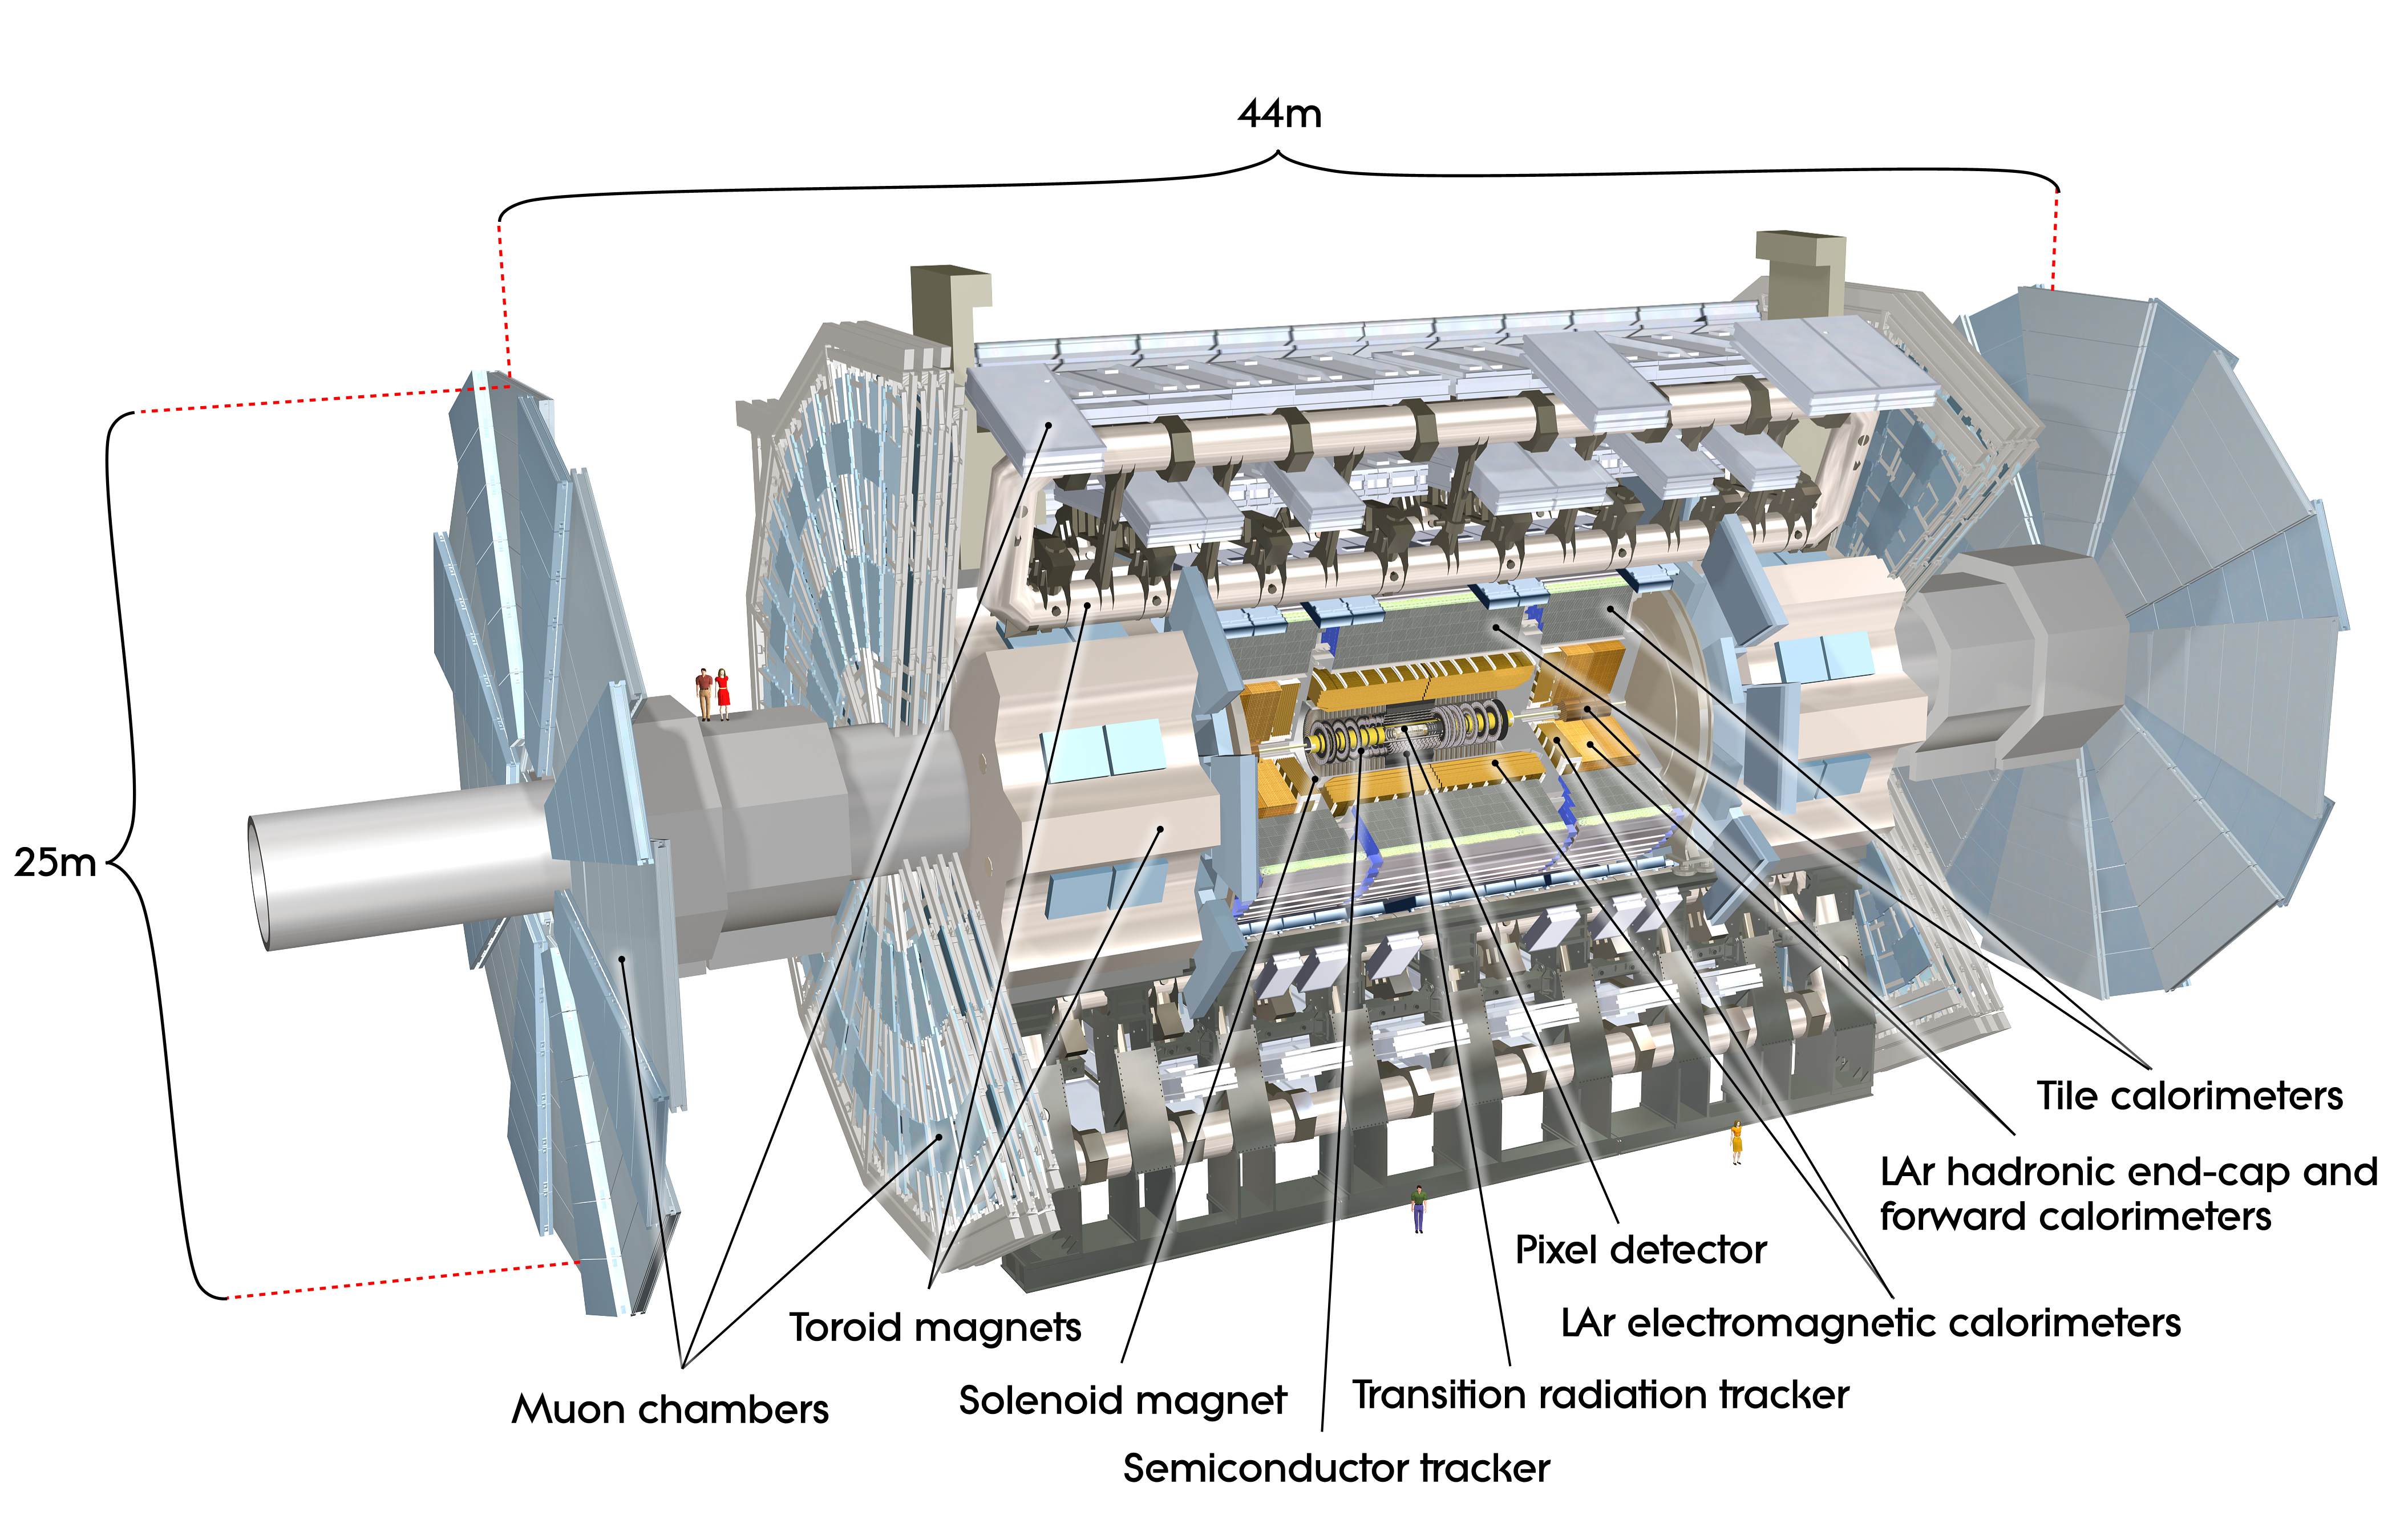
\includegraphics[width=0.85\textwidth]{figures/detector.jpg}
	\caption[]{Schematic diagram of the ATLAS detector. Source: \cite{atlas}}
	\label{fig:detector}
\end{figure}

\subsection{The Inner Detector}

The inner detector (ID), located nearest the beam pipe, is specialized for charged particle tracking. It is immersed in a 2T magnetic field oriented parallel to the beam pipe, which bends the trajectories (``tracks") of electrically charged particles as they pass through the field. Three distinct but complementary tracking technologies are employed along with pattern recognition tools to map the trajectories of charged particles passing through the ID. These reconstructed tracks are a critical component of vertex reconstruction, and the degree of bending and direction of the bent tracks at the production vertex provide information about the momentum, charge, and identity of the charged particles that produced them. 

\subsection{The Calorimeter}

The calorimeter is designed to measure the energy of all particles which pass through it by initiating ``showers" and fully absorbing their energy. The only particles which cannot be absorbed by the calorimeter are muons and neutrinos, which pass through without showering. The calorimeter is divided into two sub-detectors, the electromagnetic and hadronic calorimeters. Both are ``sampling calorimeters", which means they are comprised of repeated layers of dense absorbing material with ``sampling" layers in between. The sampling layers track the location of the shower and record a small fraction of its energy, to which a calibration factor can be applied to infer the full shower energy. 

\subsubsection{Electromagnetic Calorimeter}

The electromagnetic (EM) calorimeter forms the inner calorimeter layer, and is designed to fully absorb and measure the energies of electrons and photons. Energy is deposited in the lead absorbing layers in the form of EM showers \cite{em_showers}, in which the initial electron or photon interacts with the absorbing material to produce a cascade of photon radiation and electron pair production. The sampling layers are filled with liquid argon (LAr), with sensors to measure the ionization produced by charged particles passing through the LAr \cite{em_cal}. 

\subsubsection{Hadronic Calorimeter}

The hadronic calorimeter surrounds the EM calorimeter, and is designed to fully absorb and measure hadronic showers, also known as ``jets", initiated by hadrons, which can make it through the EM calorimeter due to their relatively long interaction length \cite{atlas}. Unlike the EM showers described above which proceed exclusively via electromagnetic interactions, hadronic showers proceed via both the strong and EM interactions, and as a result are in general more variable and less localized. 

The hadronic calorimeter is comprised of a tile calorimeter which encircles the EM calorimeter barrel, and a LAr calorimeter with copper and tungsten absorbers in the end-cap region which encloses the two ends of the barrel. The tile calorimeter uses steel as the absorber material and scintillators read out by photomultiplier tubes (PMTs) in the sampling layers. 

\subsection{The Muon Spectrometer}

The muon spectrometer \cite{atlas} surrounding the calorimeter is specialized for tracking muons and measuring their momentum. It employs the same principle used in the inner detector of applying a strong magnetic field and measuring the resulting bent trajectories of the electrically charged muons passing through to infer their momentum. 

The magnetic field is generated by rectangular superconducting ``toroid magnets" arranged azimuthally in radial planes around the beam axis, which set up a toroidal field concentric to the beam axis. In the region containing the strong field established by the toroid magnets, muon tracks are recorded by three cylindrical layers of muon tracking chambers in the barrel region and three layers of chambers arranged in wheels perpendicular to the beam axis in the end-cap region. 
%Additional layers of fast trigger chambers deliver muon track information to the ATLAS trigger system so it can be incorporated into the event readout decision. 

\section{Monte Carlo Simulation of Signal and Background}

To search for evidence of new physics in the ATLAS data, it is necessary to model the number of SM ``background" events that are expected in the selected data (see Sections 5.1 and 7 for discussions of data selection criteria used for the search), as well as their distributions in the many observables, such as \met, that can be computed from the raw data. Only the SM processes which are expected to represent statistically significant backgrounds in the selected data are considered in the analysis. The data can then be compared with the SM background model to search for evidence of an excess of events above the SM background which may be consistent with a hypothesized signal model.

Signal and SM background models are implemented by sophisticated Monte Carlo (MC) simulations of both the passage of the final-state particles through the ATLAS detector and of the physical production mechanisms. 

For a given process, for example the Z+jets background shown in figure \ref{fig:dom_bkgs}a, ``truth-level" information for each MC event is first obtained from a random proton-proton collision by simulating the physical production mechanism for the process. The set of simulated final state particles, along with their kinematic information, are collectively known as the ``truth-level" event. Truth-level events can subsequently be passed through a simulation of the ATLAS detector to model how they would actually be measured by the detector at ``reconstruction-level". 

The kinematic distributions of reconstruction-level events, scaled by the integrated LHC beam luminosity and production cross section for the process, provide a statistical model of how the given process would appear in the ATLAS data.

\section{Ongoing Search for the Dark Higgs Model in the Hadronic Decay Channel}

This section briefly summarizes the ``mono-s(WW)" search for the dark higgs model in the fully-hadronic final state channel, which is currently undergoing review within the ATLAS collaboration. MC simulated samples were generated for the dark higgs model over the grid of dark higgs and Z' boson masses shown in figure \ref{fig:had_grid}. 

 \begin{figure}[H]
	\centering
	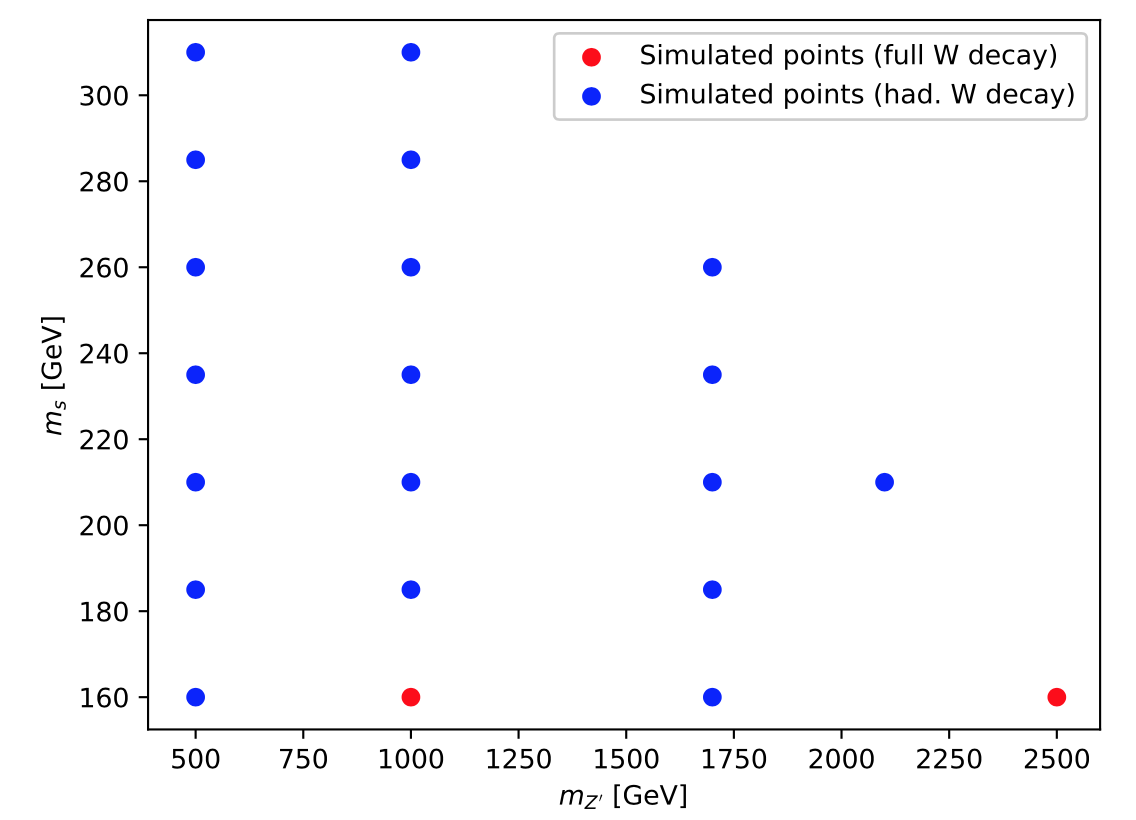
\includegraphics[width=0.7\textwidth]{figures/had_grid.png}
	\caption[]{Grid of signal models generated using MC for the hadronic mono-s(WW) analysis at various dark higgs and Z' boson masses. Red points are simulated with all three possible WW decay channels ($WW \rightarrow qqqq$, $WW \rightarrow qq\ell\nu$ and $WW \rightarrow \ell\nu\ell\nu$) and blue points are simulated exclusively with fully hadronic WW decays ($WW \rightarrow qqqq$) to save computing time.}
	\label{fig:had_grid} 
\end{figure}

\subsection{Signal Region Selection}

Selection cuts are applied to the data and MC samples in the ``signal region" (SR) with the aim of maximizing the sensitivity of the data to the dark higgs signal of interest in the fully hadronic decay channel. To avoid biasing the selection based on features in the data, the SR is `blinded', which means that the cuts are developed and optimized using the signal and background MC alone.

\subsubsection{Pre-selection}

Prior to cut optimization, loose pre-selection cuts are applied to broadly capture the region of interest for the search. As these cuts are not expected to change during subsequent optimization, they can be applied during an initial stage of data skimming to produce relatively small data files, with which further studies and optimization can be performed with reasonably fast data transfers and processing times. The pre-selection cuts used by the hadronic analysis are listed in the first column of Table \ref{tab:eventselection-baseline}, which is taken from the internal support note for the hadronic analysis. 

The first three cuts and the final cut listed in Table \ref{tab:eventselection-baseline} - 0 baseline lepton ($\ell$), \met $>$ 200 GeV, $\tau$ veto and \(N(\text{small-\(R\) jets}) \geq 2\)  - define the basic selection for a fully hadronic final state with high \met. 

A veto placed on variable radius (VR) track jets tagged as having been produced from b quarks (i.e. ``b-tagged") is designed to reduce the ``$t\bar{t}$" background of SM top quark pair production shown in figure \ref{fig:dom_bkgs}, as top quarks decay almost exclusively to b quarks. A lower bound of 15 is placed on the object based \met significance $\mathcal{S}$ with the aim of removing events with high \met originating from poor detector energy resolution. The \met significance is defined as \cite{MET_Sig}:

\begin{equation}
\mathcal{S} = \frac{\met}{\sigma_L\sqrt{1-\rho_{LT}^2}}
\end{equation}

\noindent where $\sigma_L^2$ is the measured variance of the \met in the ``longitudinal" direction parallel to the \metvec vector, and $\rho_{LT}$ is the correlation factor of momentum measurements in the directions parallel and transverse to the \metvec.

Lastly, a lower bound of 0.35 is placed on the angular separation in the plane transverse to the beam line between each of the leading three small-radius jets and the \metvec to select for the desired topology of DM recoiling against jets. Note that some events may contain only two small-radius jets, in which case the lower bound on $\Delta\phi_\text{jets, \met}$ is applied only to these two jets.

\begin{table}[ht]
    \centering
    \caption{The pre-selection which is required in the signal and control regions.}
    \label{tab:eventselection-baseline}
    \resizebox{\textwidth}{!}{%
    \begin{tabular}{ccc}
    \toprule
    0 \(\ell\) SR & 1 \(\mu\) control region & 2 \(\ell\) control region \\ \midrule
    0 baseline \(\ell\) & 0 baseline e,  1 baseline+signal \(\mu\) & 2 baseline+signal \(ee\) / opposite sign \(\mu^{+} \mu^{-}\) \\
    \met $>$ 200 GeV  & \metnomu $>$ 200 GeV & \ptll $>$ 200 GeV\\
    \(\tau\) veto & \(\tau\) veto & \(\tau\) veto \\
    0 \(b\)-tagged VR track jets in event & 0 \(b\)-tagged VR track jets in event & 0 \(b\)-tagged VR track jets in event\\
    VR track jet \(\Delta R\) overlap veto & VR track jet \(\Delta R\) overlap veto & VR track jet \(\Delta R\) overlap veto \\
    \(\mindphi > 0.35\) & \(\mindphi > 0.35\) & - \\

    \(\mathcal{S} > 15\) & \(\mathcal{S} > 15\) & \(\mathcal{S} < 15\) \\
    \(N(\text{small-\(R\) jets}) \geq 2\) &  \(N(\text{small-\(R\) jets}) \geq 2\) &  \(N(\text{small-\(R\) jets}) \geq 2\)
    \\ \bottomrule
    \end{tabular}}
\end{table}

\subsubsection{Kinematic Categories}

In addition to the pre-selection cuts described in Section 5.1.1, further selections are optimized separately in the three kinematic categories illustrated in figure \ref{fig:had_categories}, known as ``merged", ``intermediate" and ``resolved". 

\begin{figure}[H]
     \centering
     \begin{subfigure}[b]{0.29\textwidth}
         \centering
         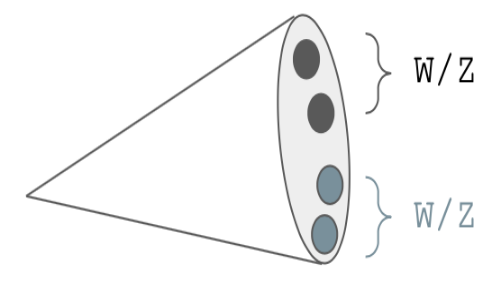
\includegraphics[width=0.95\textwidth]{figures/had_merged.png}
         \caption[]{Merged category}
         \label{fig:had_merged}
     \end{subfigure}
     \hfill
     \begin{subfigure}[b]{0.29\textwidth}
         \centering
         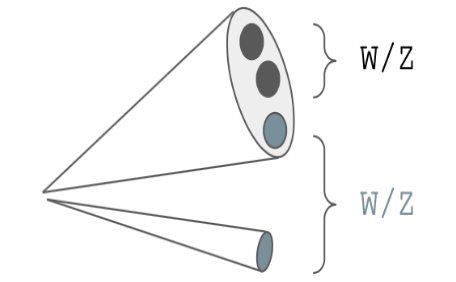
\includegraphics[width=0.95\textwidth]{figures/had_int.png}
         \caption[]{Intermediate category}
         \label{fig:had_int}
     \end{subfigure}
     \hfill
     \begin{subfigure}[b]{0.29\textwidth}
         \centering
         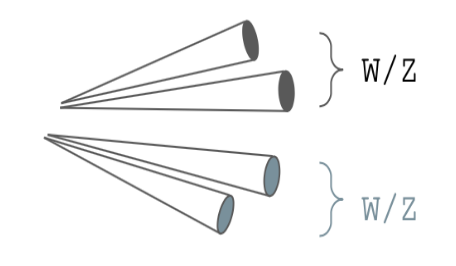
\includegraphics[width=0.95\textwidth]{figures/had_resolved.png}
         \caption[]{Resolved category}
         \label{fig:had_resolved}
     \end{subfigure}
\caption[]{Illustration of the kinematic categories used for event selection optimization in the analysis of the mono-s(WW) hadronic channel. Source: Adapted from a figure shown by P. Gadow in an ATLAS internal approval presentation. }
\label{fig:had_categories}
\end{figure}

The ``merged" category represents a regime in which the hadronic final state is sufficiently boosted in the transverse plane that the quark hadronizations identified as having originated from the hadronic WW decays cannot be individually resolved, and are instead reconstructed as a single large-radius jet. In the ``resolved" category, the boost is sufficiently small that all four quark hadronizations identified as having originated from W decays can be resolved into individual jets. In between these two extremes is the ``intermediate" category, which is characterized by two or three of the hadronized quarks being reconstructed together as a large-radius (large-R) jet and the others being resolved into individual jets.

\subsection{Control Regions}

Control regions (CRs) are designed to provide data-driven normalization constraints for the dominant Z+jets and W+jets SM background processes, shown in figure \ref{fig:dom_bkgs}. The CR is chosen by selecting a region of phase space that is kinematically similar to the SR, and which contains a high purity of the background process to be normalized. The CR must be orthogonal to the SR to avoid unblinding any part of the SR. To minimize the possibility of any signal events in the data affecting the normalization of the SM background process, it is also desirable to select a CR in which negligible contamination of the MC signal events is observed. Data and MC distributions are compared in the intermediate kinematic category of the two CRs in figure \ref{fig:had_Intermediate_DataMC}. 

\begin{figure}[H]
     \centering
     \begin{subfigure}[b]{0.4\textwidth}
         \centering
         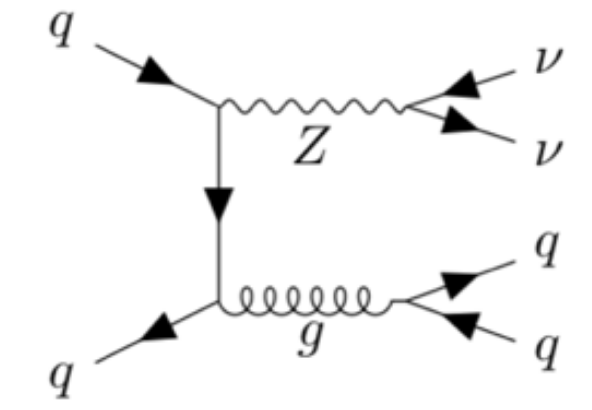
\includegraphics[width=0.9\textwidth]{figures/Zjet_feynman.png}
         \caption[]{Z+jets}
         \label{fig:zjets}
     \end{subfigure}
     \hfill
     \begin{subfigure}[b]{0.4\textwidth}
         \centering
         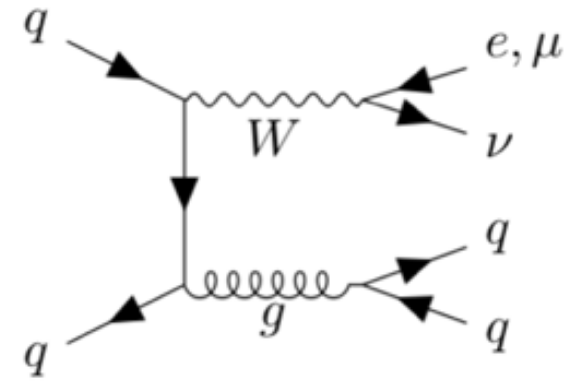
\includegraphics[width=0.9\textwidth]{figures/Wjet_feynman.png}
         \caption[]{W+jets}
         \label{fig:wjets}
     \end{subfigure}
     \hfill
     \begin{subfigure}[b]{0.4\textwidth}
         \centering
         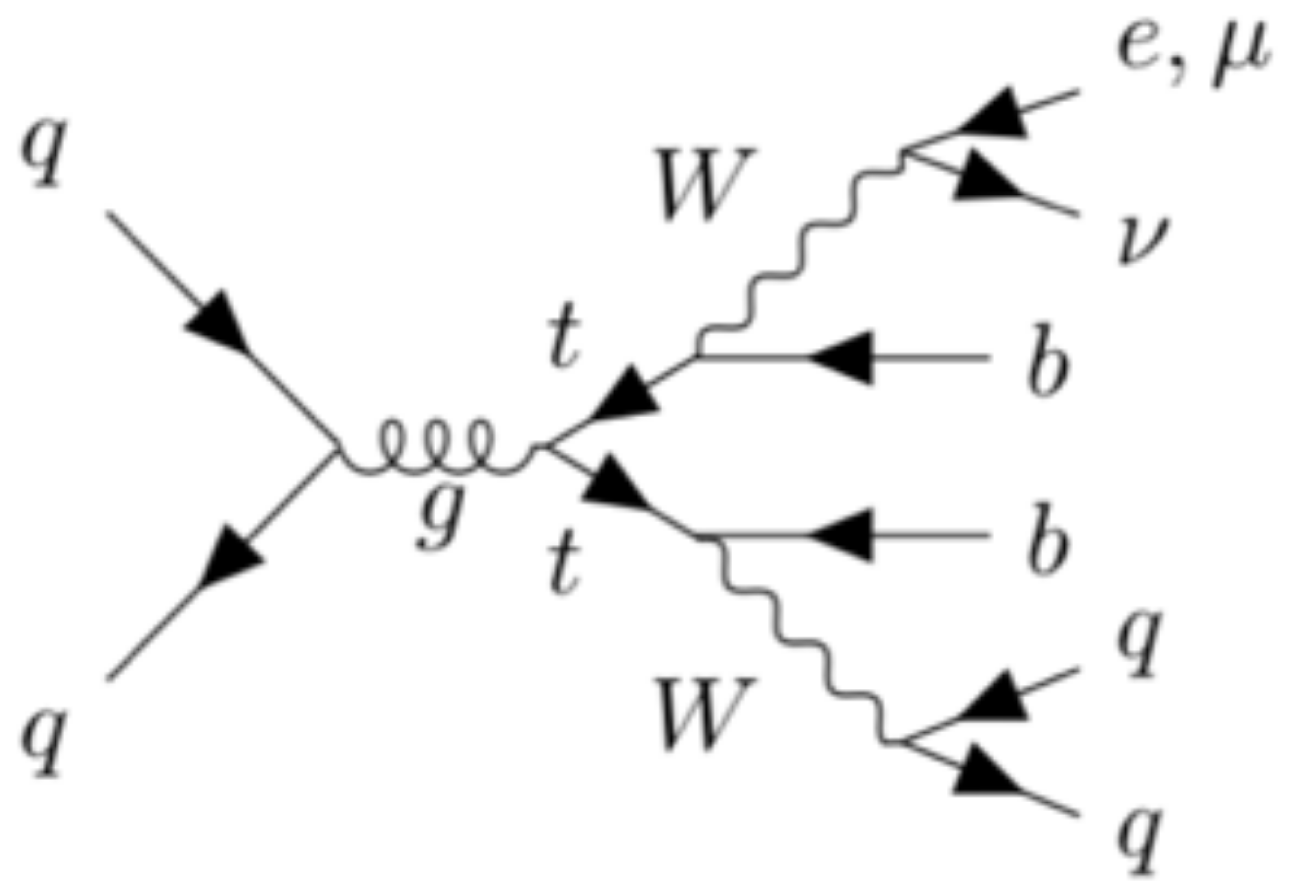
\includegraphics[width=0.9\textwidth]{figures/ttbar_feynman.png}
         \caption[]{$t\bar{t}$}
         \label{fig:ttbar}
     \end{subfigure}
\caption[]{Dominant SM background processes for the mono-s(WW) search. The Z+jets background is only dominant in the hadronic channel, as it is significantly reduced by the 1-lepton requirement in the semileptonic channel.}
\label{fig:dom_bkgs}
\end{figure}

\begin{figure}[H]
	\centering
	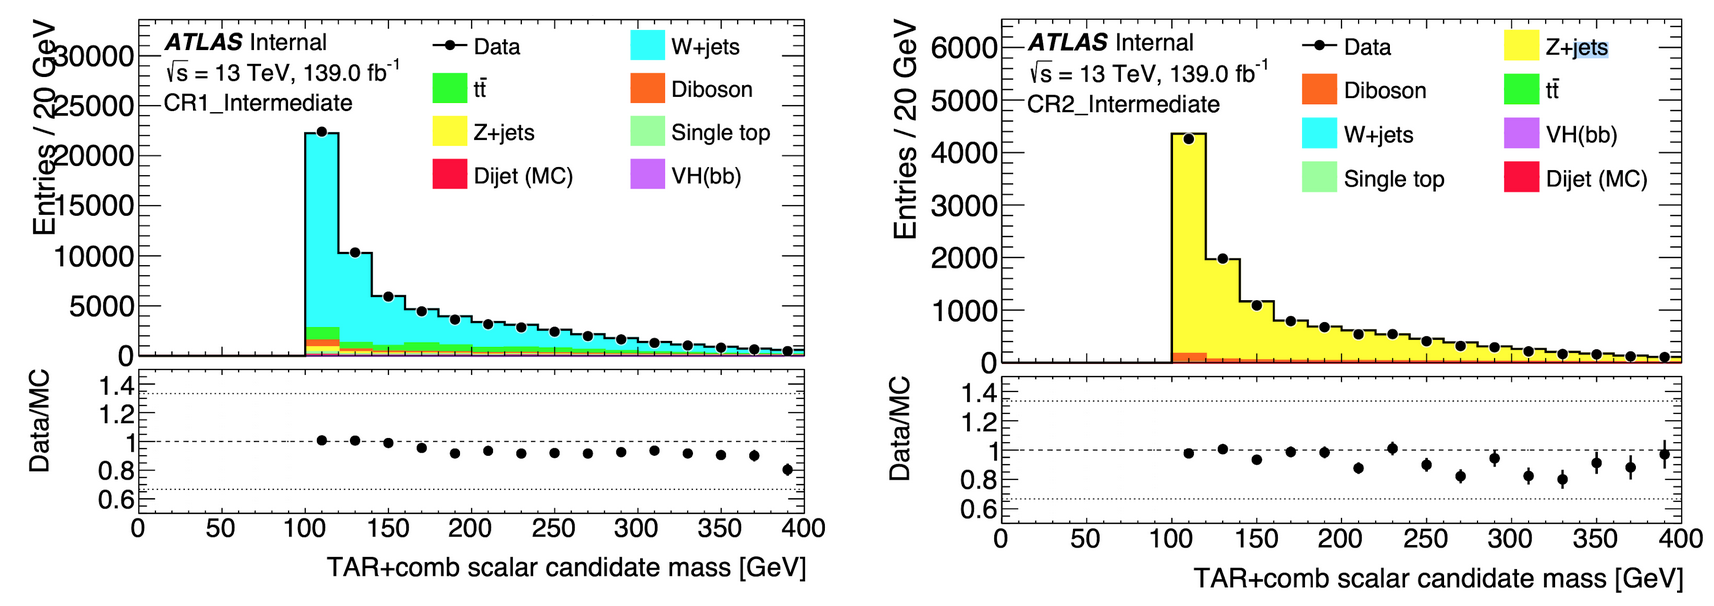
\includegraphics[width=\textwidth]{figures/had_Intermediate_DataMC.png}
	\caption[]{Data-MC comparisons of reconstructed dark higgs candidate mass distributions in the intermediate kinematic category of the 1-lepton (left) and 2-lepton (right) CRs}.
	\label{fig:had_Intermediate_DataMC} 
\end{figure}

\subsubsection{1 Lepton CR}

The 1 lepton CR is identical to the SR, except that the lepton veto is replaced by a requirement of one signal muon. This CR is designed to obtain a purified sample of the SM W+jets background in which the \met arises from a neutrino produced in the leptonic decay of a W boson, and thereby provide a constraint on the normalization of this background process. In the fully hadronic SR, the lepton in this process is not properly reconstructed, and escapes detection. 

\subsubsection{2 Lepton CR}

The 2 lepton CR is also largely identical to the SR. The primary difference is the replacement of the lepton veto in the SR by a requirement of two signal muons or electrons in the CR. This CR is designed to obtain a purified sample of the Z+jets background in the case where the Z decays leptonically ($Z\rightarrow\ell\ell$). This sample is used to obtain a normalization factor for the Z+jets background in the SR, where the Z decays are predominantly hadronic ($Z\rightarrow qq$), by making use of existing high-precision measurements of the relative production cross sections of these two Z decay channels. In addition to the two-lepton requirement, the \met significance cut is reversed in the 2 lepton CR and the \mindphi cut is removed to boost the contribution from QCD background. 

\subsection{Systematic Uncertainties}

In addition to the statistical uncertainty arising from the limited number of events present in the data and simulated in the MC, systematic uncertainties arising from both theoretical and experimental sources can affect the normalization and shape of observables used in the analysis. These systematic uncertainties are evaluated as variations in the weights associated with MC generated events. The weight variations are produced by varying MC input parameters from their nominal values by their respective systematic uncertainty. 

\subsubsection{Experimental systematics}

Experimental systematic uncertainties arise from various aspects of modelling the ATLAS detector and LHC machine, and are provided by the relevant ATLAS performance groups. These include the limited precision of our knowledge of the LHC beam luminosity, uncertainties associated with lepton and muon reconstruction and identification, and jet energy resolution. Uncertainties associated with the reconstruction of the \met are also considered. 

\subsubsection{Theoretical Modelling Uncertainties}

Theoretical modelling uncertainties associated with MC event generation are evaluated both for signal and for the dominant Z+jets and W+jets SM background processes. Variations arising from the modelling of the parton density functions (PDFs) \cite{PDG_PDF} of the colliding protons are considered, along with the renormalization and factorization scales \cite{PDG_QCD} used to model QCD processes. 

For the W+jets and Z+jets background processes, which are nominally modelled with the SHERPA generator \cite{SHERPA}, the variation arising from generating the events with an alternative event generator called PYTHIA 8 \cite{PYTHIA8} is also considered. The alternative generator uses a different algorithm to model parton showering, with all other settings in the alternative generator kept the same. 

\subsection{Sensitivity Estimates}

To estimate the sensitivity of the search in the hadronic channel, the data is binned in \met and dark higgs candidate mass. Mock binned data is generated for each signal point to be statistically consistent with the simulated SM background. The SM background and signal model are then fit to this mock background-only data for events passing the event selection criteria. The W+jets and Z+jets background shapes are obtained from MC, and their normalization factors from the 1-lepton and 2-lepton CRs, respectively. 

The fit is used to obtain a CLs value \cite{PDG_stats} for each signal point, defined as:

\begin{equation}
\text{CLs} = \frac{p_\mu}{1-p_\text{b}}
\end{equation}

\noindent where p$_\mu$ is the p-value of the background+signal hypothesis and p$_\text{b}$ is the p-value of the background-only hypothesis. 

The CLs can also be expressed as a ``significance" by treating the CLs as a p-value and computing the corresponding standard deviation from the null background-only hypothesis. Signal points with CLs value below 0.05, or significance above 1.96, could be excluded for the hypothesized production cross section with 95\% confidence if the data is statistically consistent with the background. 

\begin{figure}[H]
     \centering
     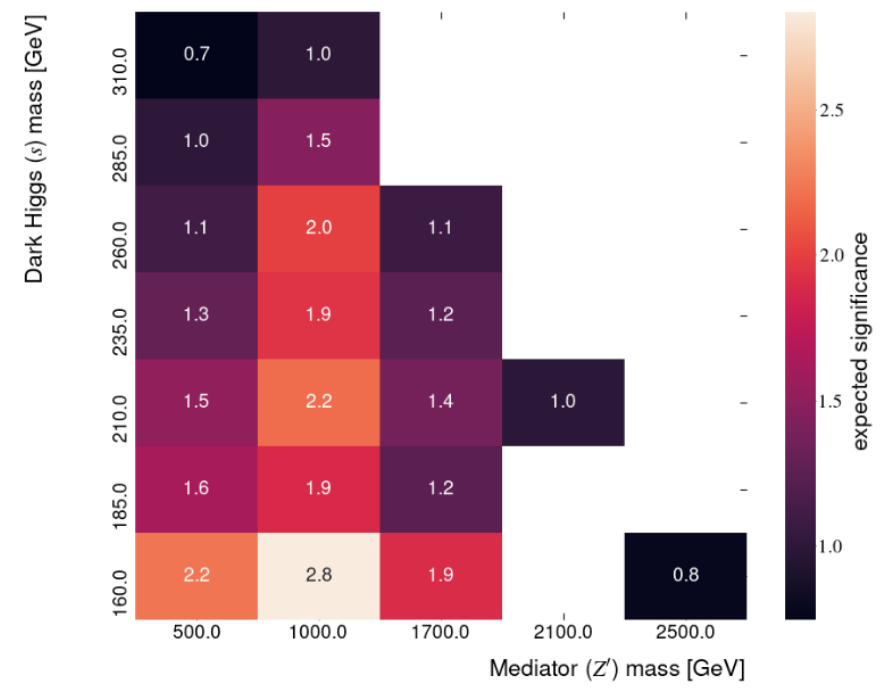
\includegraphics[width=0.6\textwidth]{figures/had_sensitivity.png}
\caption[]{Sensitivity estimate for hadronic channel, expressed in terms of significance. The fit includes all analysis regions and systematic uncertainties.}
\label{fig:sensitivity}
\end{figure}

\section{Search for the Dark Higgs Model in the Semileptonic Decay Channel}

The proposed thesis will focus on the search for the dark higgs model in the semileptonic $WW\rightarrow qq\ell\nu$ decay channel. This section summarizes the current status of ongoing analysis work in this channel. 

\subsection{Signal Sample Generation}

\subsubsection{Parameter Choices}

MC signal samples for the dark higgs model with s$\rightarrow$WW decay are generated over a range of m($s$) and m($Z'$) for which the analysis is expected to be sensitive to the model. There are several other free parameters in the dark higgs model which need to be fixed to perform the scan. The parameter choices are identical to those used for the re-interpreted mono-H(bb) search described in Section 2.4.1:

\begin{itemize}
	\item Coupling $g_{q}$ of the Z' boson to quarks: 1 
	\item Coupling $g_{\chi}$ of the Z' boson to DM: 0.25
	\item DM mass $m_{\chi} = 200$ GeV
	\item Mixing angle $\theta$ between the SM and dark sector higgs bosons: 0.01
\end{itemize}

The values of $g_q$, $g_\chi$ and $m_\chi$, listed above are standard choices used by many other LHC searches. The use of standard parameter choices facilitates comparisons and combinations of search results between different analyses. The value of $\theta$ was chosen from the approximate range of 0.01-0.1 suggested by the authors of the phenomenology paper \cite{dark_higgs} in which the model is introduced. It is discussed in the paper that the precise value of the mixing angle is not important for the analysis. It need only be sufficiently large that the dark higgs will decay promptly and sufficiently small as to avoid constraints from existing measurements of the SM Higgs couplings \cite{Aad_2016}. 

\subsubsection{Semileptonic Signal Grid}

A signal grid has been generated for the mono-s(WW) signal with semileptonic WW decay, presently at the same points that were generated with hadronic decay for the hadronic analysis described in Section 5. There are additionally two signal points generated with all possible WW decay modes (i.e. `inclusive'). 

Work is ongoing to re-generate the grid with a more recent release of the ATLAS simulation software, and extend it as shown in Fig. ~\ref{fig:signalgrid} to allow for a more complete coverage of the phase space region to which the analysis could be sensitive.

\begin{figure}[H]
	\centering
	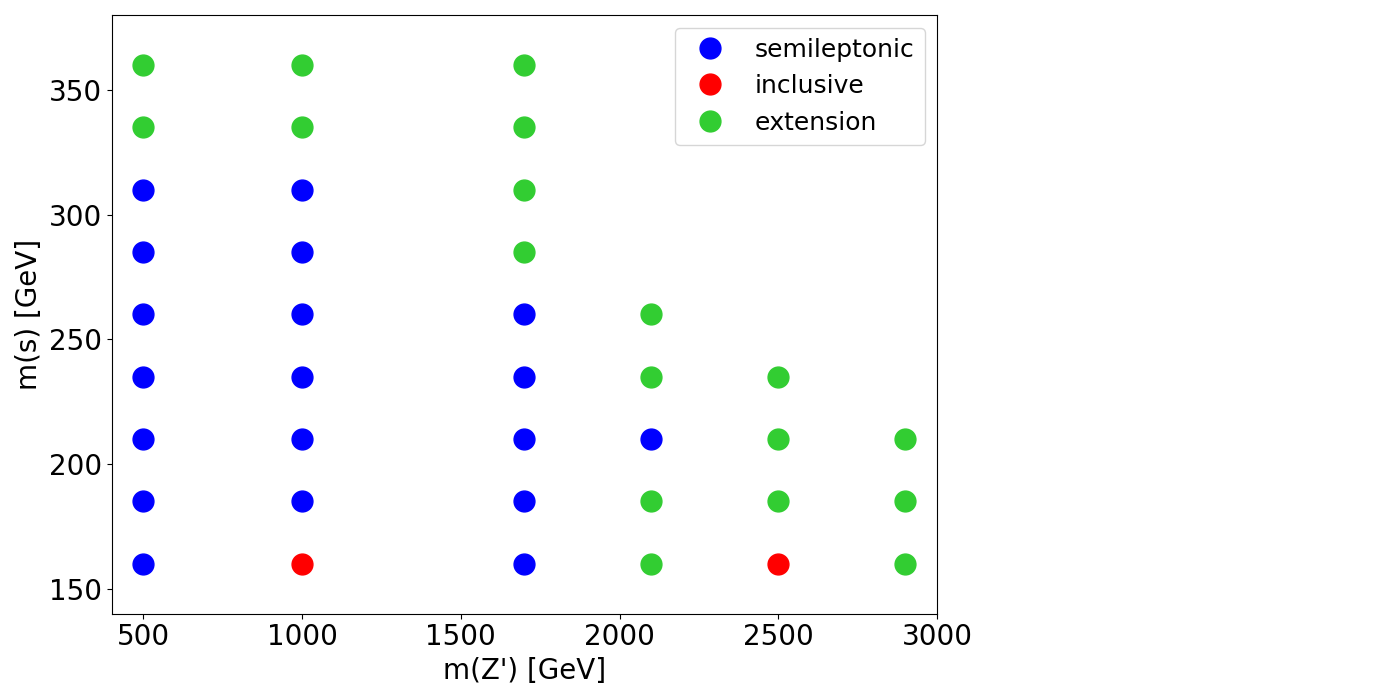
\includegraphics[width=0.7\textwidth]{figures/SignalGrid_simple.png}
	\caption[]{Grid of signal points with respect to dark higgs (s) and $Z'$ boson masses}
	\label{fig:signalgrid}
\end{figure}

\subsection{Event Selection for the Semileptonic Channel}

This section describes the current event selection used to optimize the sensitivity of the analysis to the dark higgs signal with semileptonic WW decay. The selection is in the process of being refined, so many details presented here are preliminary and will likely evolve as the ongoing refinements progress. 

\subsubsection{Pre-selection}

As was done for the hadronic analysis, several pre-selection cuts are applied to broadly define the channel prior to further cut optimization. The current pre-selection cuts are listed below.

\begin{itemize}
\item Event passes \met trigger
\item 1 signal muon or 1 signal electron
\item \met $>$ 150 GeV
\end{itemize}

In addition to the current pre-selection cuts, the following two cuts are common to both kinematic categories of the signal region (see Section 6.2.2), and may become listed as pre-selection in the future:

\begin{itemize}
\item Veto on b-tagged jets
\item Lepton-\met transverse mass $m_T(\ell, \met)$ $>$ 150 GeV
\end{itemize}

The transverse mass $m_T(\met, \ell)$ between the lepton and \met is considered in the semileptonic channel, because it is sensitive to the presence of additional \met beyond that arising from the neutrino in the semileptonic W decay. It is computed in the ATLAS data and MC as:

\begin{equation}
m_T(\ell, \met) = \sqrt{2p_{T, \ell} \met(1-\cos\theta_{\ell, \met})}
\end{equation}
which comes from the full transverse mass definition \cite{PDG_kin}

\begin{equation}
m_{T, \text{ full}}^2(\ell, \met) = (E_{T, \ell}^2 + E_{T, \met}^2 - (p_{T, \ell}^2 + p_{T, \met}^2)) 
\end{equation}

$$
= m_\ell^2+m_{\met}^2 + 2E_{T, \ell}, E_{T, \met}(1-\cos\theta_{\ell, \met})
$$
under the assumptions that the masses associated with the lepton and \met are negligibly small compared with their momenta. The assumption of negligible lepton mass is in general justified given the energy of LHC collisions. The assumption of negligible mass associated with \met is justified if the true \met arises only from the neutrino in the semileptonic W decay, as it would in the leading SM backgrounds. In the signal model, however, there is additional mass associated with the \met arising from DM production. The result, shown in figure \ref{fig:mT_lep_met} after applying the pre-selection cuts, is that the bulk of the SM background has $m_T(\ell, \met)$ below the W mass peak, but the signal distribution tends to be peaked closer to $\sim$250 GeV. 

\begin{figure}[H]
	\centering
	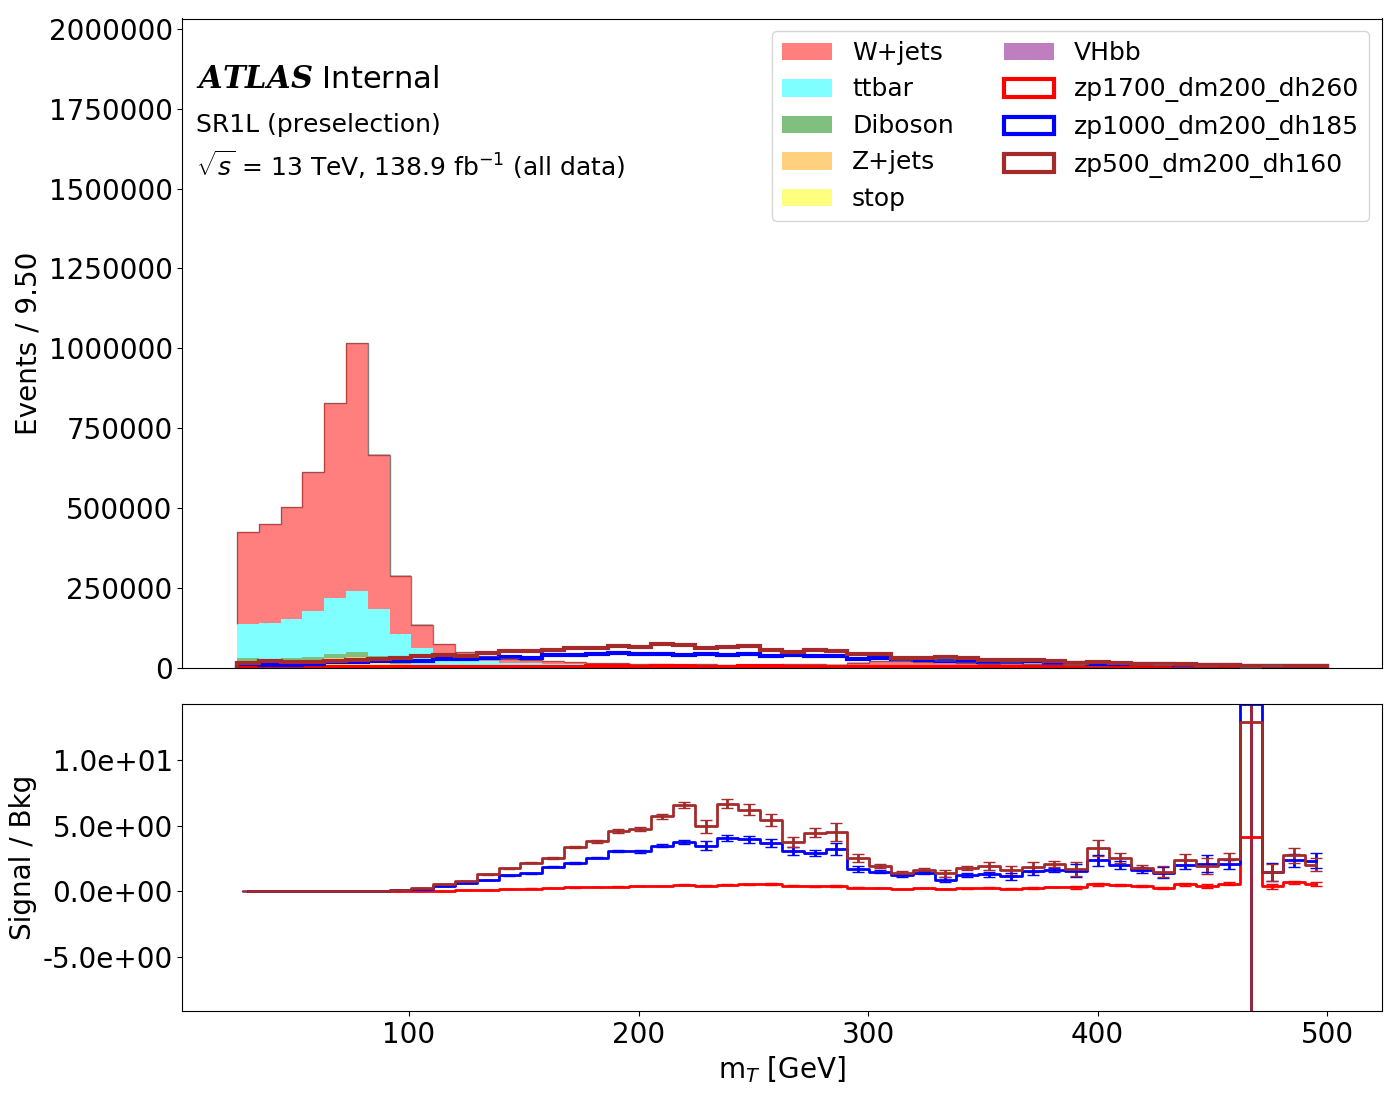
\includegraphics[width=0.7\textwidth]{figures/mT_lep_met_preselection.png}
	\caption[]{Transverse mass distribution for SM background and several signal points with pre-selection cuts}
	\label{fig:mT_lep_met}
\end{figure}

\subsubsection{Kinematic Categories}

Further cuts are optimized within the two kinematic categories illustrated in figure \ref{fig:lep_categories}. As in the hadronic analysis, the kinematic category definitions aim to characterize the degree to which the leading hadronic jets in the event are boosted. The ``merged" category aims to capture the highly boosted regime, in which the final state is sufficiently boosted in the transverse plane that the leading hadronic showers are reconstructed as a single large-radius jet. The ``resolved" category captures the regime in which all hadron showers have a low enough boost as to be individually reconstructed as small-radius jets. In both categories, there is a possibility of overlap between the leptonic and hadronic decay products. Studies are ongoing to improve the algorithm used for disentangling the final-state lepton from jets for events in which such overlap occurs - see Section 8.2 for details. 

The intermediate category used in the hadronic analysis, characterized by a combination of large- and small-radius jets, is not considered for the semileptonic channel because the semileptonic WW decay in the signal model produces only two final-state quarks. 

\begin{figure}[H]
     \centering
     \begin{subfigure}[b]{0.4\textwidth}
         \centering
         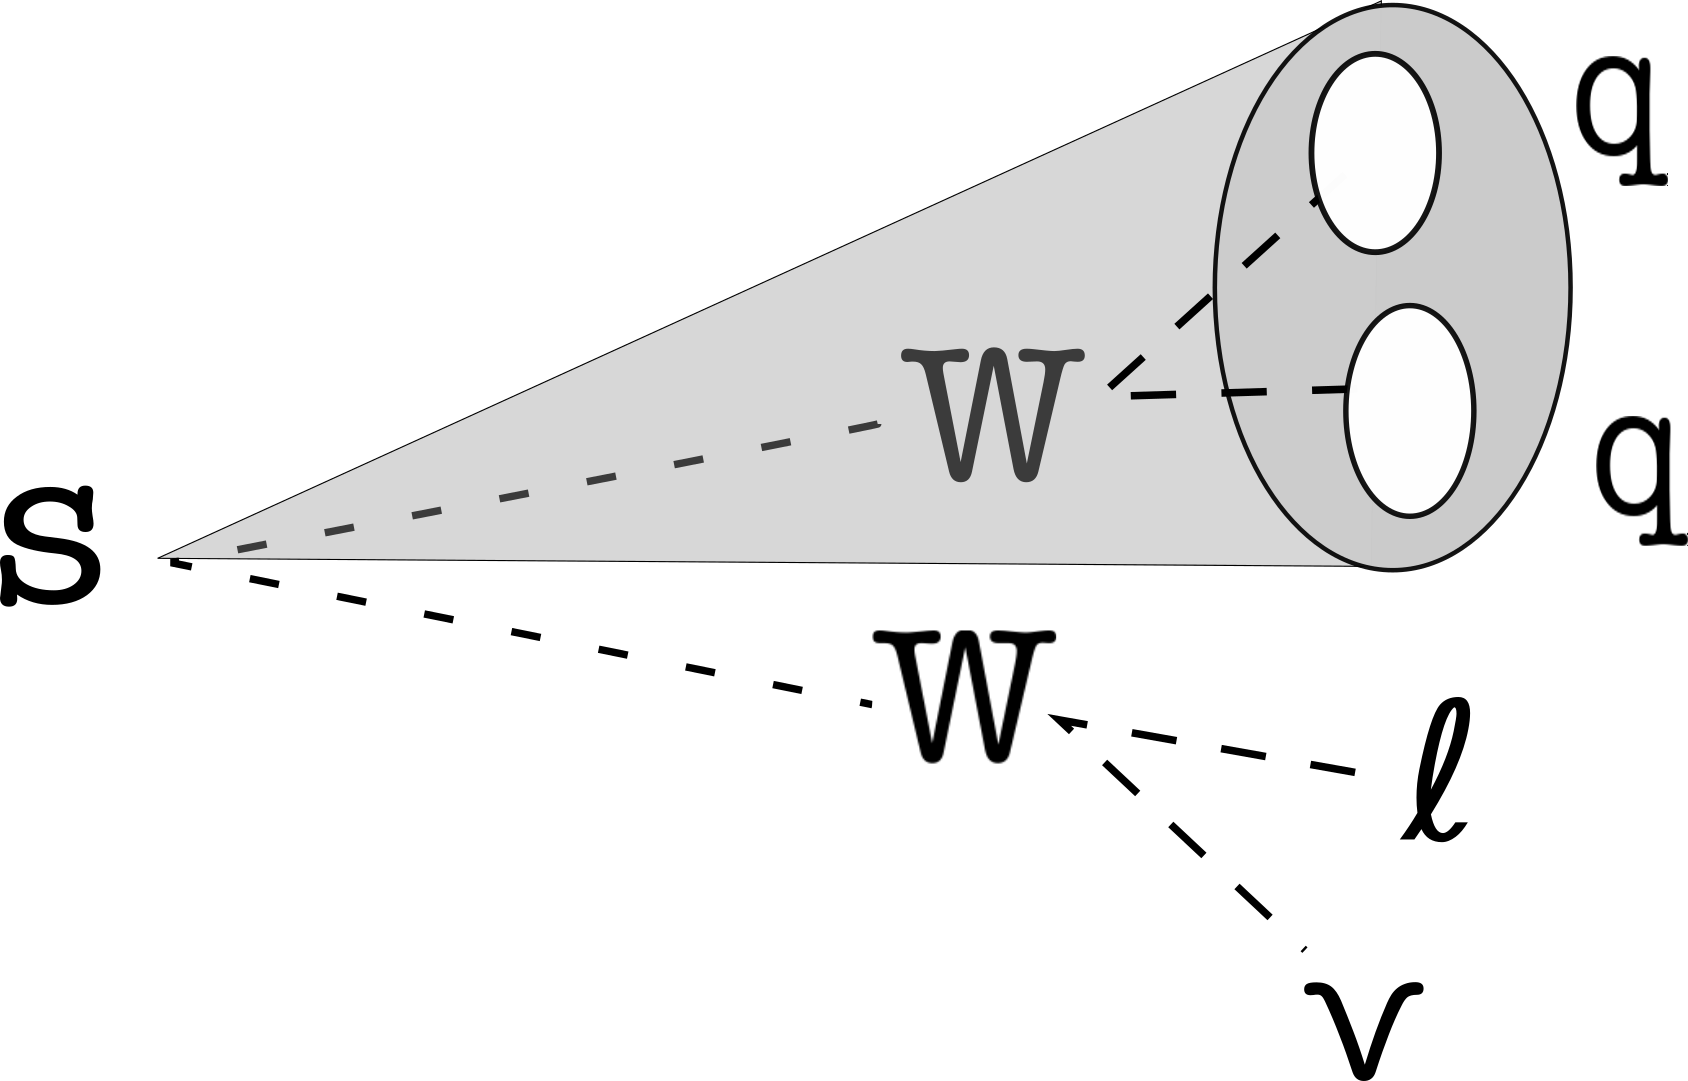
\includegraphics[width=0.9\textwidth]{figures/merged.png}
         \caption[]{Merged category}
         \label{fig:merged}
     \end{subfigure}
     \hfill
     \begin{subfigure}[b]{0.4\textwidth}
         \centering
         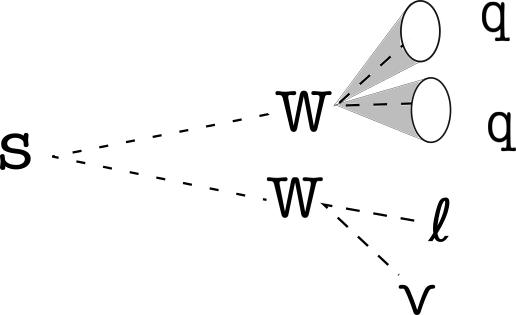
\includegraphics[width=0.9\textwidth]{figures/resolved.png}
         \caption[]{Resolved category}
         \label{fig:resolved}
     \end{subfigure}
\caption[]{Kinematic categories for the semileptonic WW decay channel}
\label{fig:lep_categories}
\end{figure}

The current merged and resolved category cut definitions, listed and discussed in tables \ref{tab:merged_cuts} and \ref{tab:resolved_cuts} respectively, have been developed and optimized by two other members of the analysis team. The \met distributions for each category are shown in figure \ref{fig:met_categories}. There is ongoing work within the analysis team to investigate the benefit of tuning the selection further by optimizing the selections within the $WW\rightarrow qqe\nu$ and $WW\rightarrow qq\mu\nu$ decay channels separately.

\begin{figure}[H]
     \centering
     \begin{subfigure}[b]{0.49\textwidth}
         \centering
         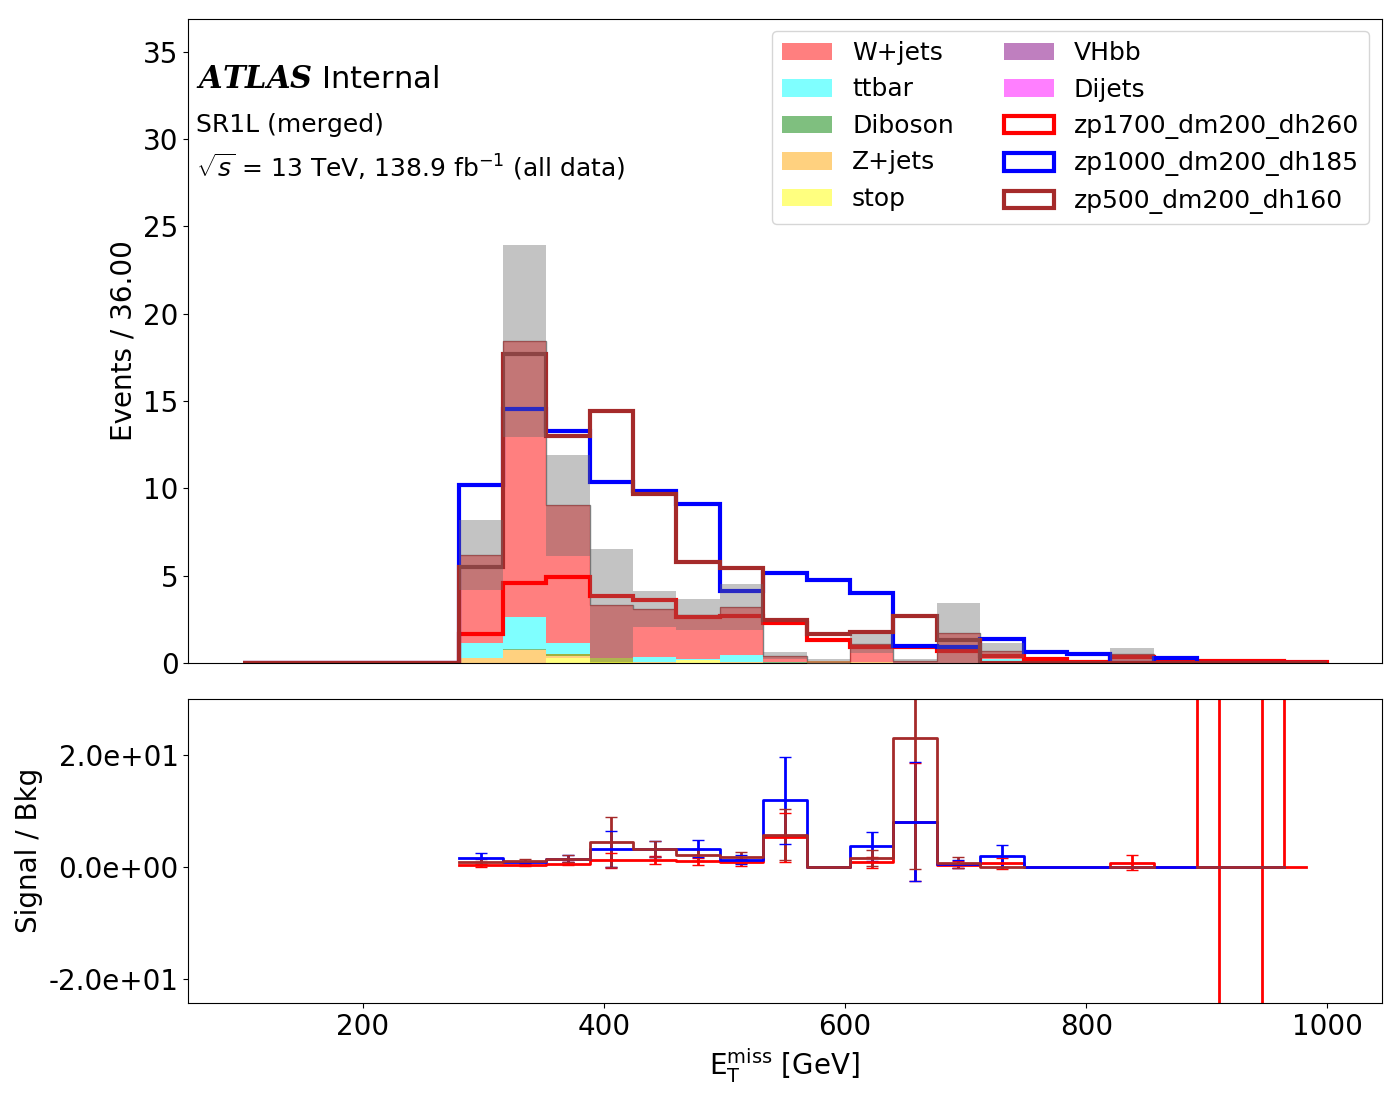
\includegraphics[width=\textwidth]{figures/MetTST_met_merged.png}
         \caption[]{Merged category (cuts listed in Table \ref{tab:merged_cuts})}
         \label{fig:merged}
     \end{subfigure}
     \hfill
     \begin{subfigure}[b]{0.49\textwidth}
         \centering
         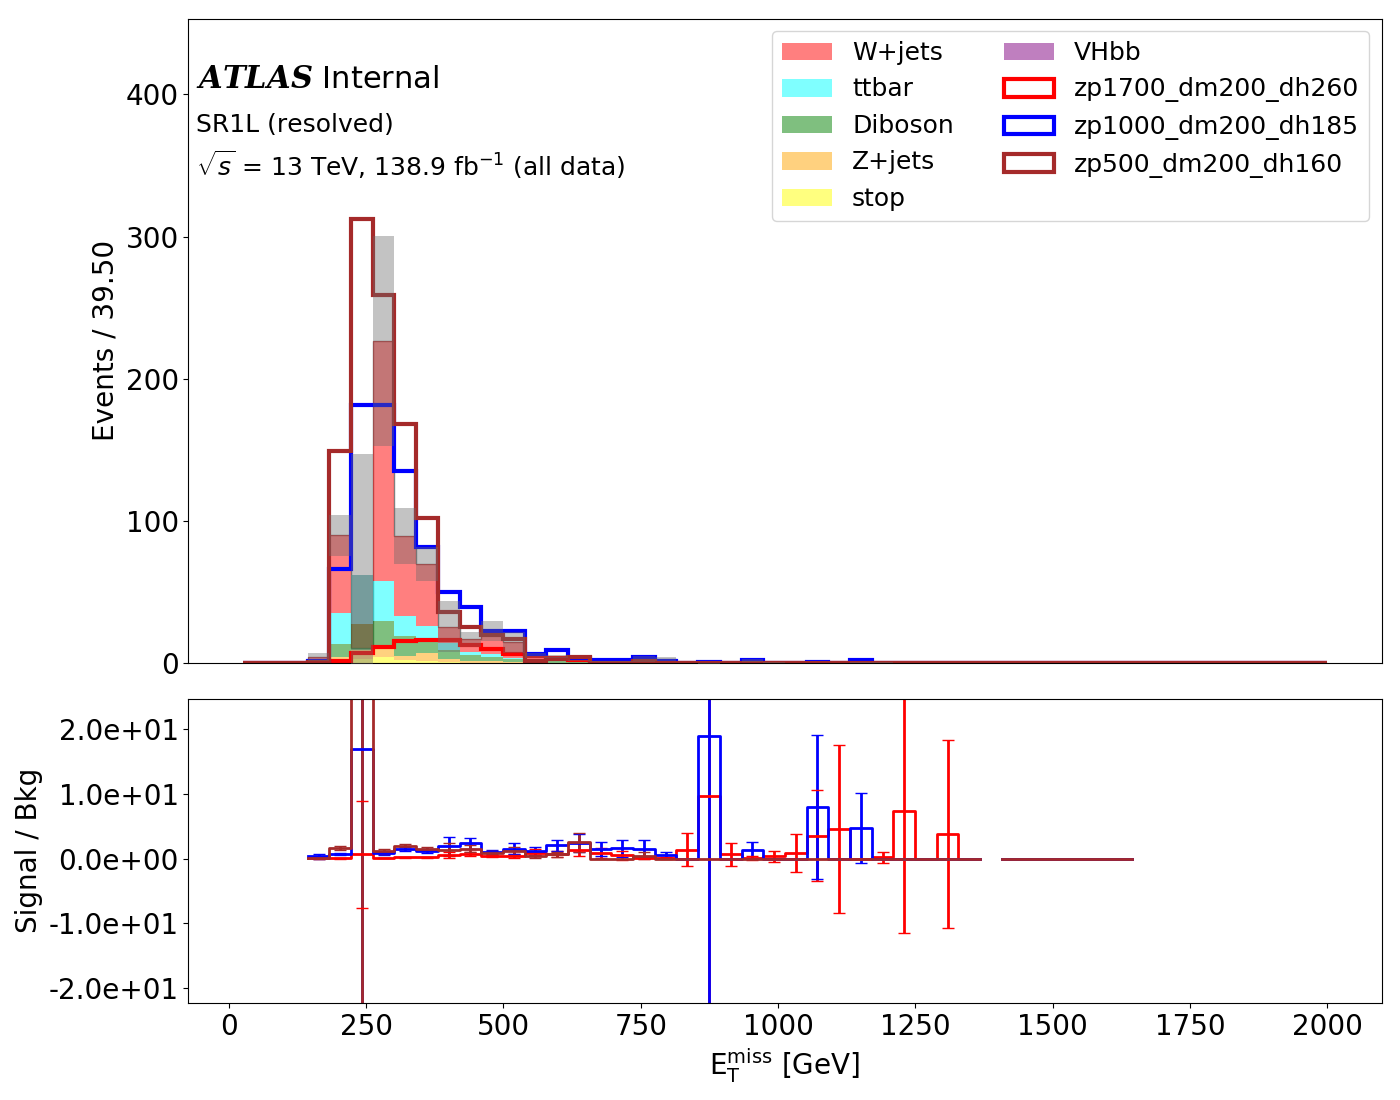
\includegraphics[width=\textwidth]{figures/MetTST_met_resolved.png}
         \caption[]{Resolved category (cuts listed in Table \ref{tab:merged_cuts})}
         \label{fig:resolved}
     \end{subfigure}
\caption[]{\met distributions in the SR in the two kinematic categories developed for the semileptonic WW decay channel. Signals are shown with amplitudes multiplied by a factor of 2. Grey bands represent statistical uncertainty.}
\label{fig:met_categories}
\end{figure}

\begin{table}[H]
\centering
\caption{Current data selection cuts in the \textbf{merged} category of the semileptonic decay channel}
\label{tab:merged_cuts}
\begin{footnotesize}
\renewcommand{\arraystretch}{1.5}
\begin{tabular}{|p{50mm}|p{100mm}|}
\hline
\textbf{Selection} & \textbf{Discussion}  \\ \hline
Pre-selection & Listed in Section 6.2.1      \\ \hline
At least 1 large-radius jet & -      \\ \hline
\met $>$ 300 GeV      & -      \\ \hline
Reconstructed mass of large-radius jet $\in$ [60 GeV, 100 GeV]     & Increases the likelihood that the selected large-R jet originates from a W boson.        \\ \hline
\met significance $>$ 15    &  -        \\ \hline
$\Delta R(\ell$, large-R jets) $<$ 1.6    & $\Delta R = \sqrt{\Delta\phi^2+\Delta\eta^2}$ is the angular distance between the lepton and the large-radius jet, where $\Delta\phi$ is the angular separation in the transverse plane and pseudorapidity $\eta$ is a quantity related to the angle $\theta$ of a particle relative to the beam axis: $\eta=-\ln\Big[\tan\Big(\frac{\theta}{2}\Big)\Big]$. Pseudorapidity is used rather than $\theta$ because differences $\Delta\eta$ in pseudorapidity are invariant under lorentz boosts. An upper bound is placed on the angular distance to select for the boosted topology of interest, in which all decay products of the dark higgs boson are boosted in approximately the same direction.      \\ \hline
$D_{2}$ of leading large-R jet $<$ 1.4   & The $D_{2}$ variable \cite{Marzani_2019} uses energy correlation functions to give a measure of the likelihood that a jet contains only two spatially separated energy sources. This allows the semileptonic signal channel - in which only two dominant energy sources (i.e. ``prongs") would be expected due to the $W\rightarrow qq$ decay - to be separated from the QCD background which may contain many such prongs.     \\ \hline
\end{tabular}
\end{footnotesize}
\end{table}

\begin{table}[H]
\centering
\caption{Current data selection cuts in the \textbf{resolved} category of the semileptonic decay channel}
\label{tab:resolved_cuts}
\begin{footnotesize}
\renewcommand{\arraystretch}{1.5}
\begin{tabular}{|p{50mm}|p{100mm}|}
\hline
\textbf{Selection} & \textbf{Discussion}  \\ \hline
Pre-selection & Listed in Section 6.2.1      \\ \hline
At least 2 small-radius jets & -     \\ \hline
Reconstructed mass of the $W$ candidate $\in$ [60 GeV, 100 GeV]     & The W candidate is selected by considering all combinations of small-radius jets, and identifying the pair whose reconstructed mass is closest to the W boson mass of 80.4 GeV.        \\ \hline
\met significance $>$ 13    & -        \\ \hline
$m_T(\ell, \met)$ $>$ 200 GeV    & -        \\ \hline
 $W$ candidate $p_T$ $>$ 100 GeV    & The lower bound on the W candidate $p_T$ increases the likelihood that the two jets used to reconstruct the W boson actually originated from the decay of a boosted parent particle.   \\ \hline
$\Delta R(W, \ell) < 1$   & An upper bound on the angular distance between the $W$ boson candidate and the lepton selects for the topology of interest in which one of the boosted $W$ bosons decays leptonically, such that in the lab frame, the lepton is expected to be measured in approximately the same direction as the reconstructed $W$.   \\ \hline
\end{tabular}
\end{footnotesize}
\end{table}

\subsubsection{W+jets Control Region}

The W+jets CR is defined with the aim of providing a data-driven estimate of the normalization of the W+jets background, illustrated in figure \ref{fig:wjets}, in the SR. The exact definition of this CR is still being studied and optimized, but at its simplest, it would reverse only the transverse mass cut: 

$$
m_T(\ell, \met)>150\text{ GeV} \rightarrow 50\text{ GeV} \leq m_T(\ell, \met)\leq 150\text{ GeV}
$$

This reversal makes the W+jets CR orthogonal to the SR, and aims to boost the statistics and purity of the W+jets background without drastically changing the kinematics of the region. Table \ref{tab:crw_info} shows that the $m_T(\ell, \met)$ cut reversal improves the W+jets purity with very low signal contamination, but only improves the W+jets statistics in the resolved category. The signal fraction in table \ref{tab:crw_info} is defined as:

\begin{equation}
\text{signal fraction} = 100\% \times \frac{\sum \text{signal events}}{\sum \text{background events}}
\end{equation}

\begin{table}[H]
\centering
\caption{Comparison of W+jets CR performance measures between SR and preliminary W+jets CR. Signal fraction is averaged over all signal points, and uncertainty is the standard deviation among all points.}
\label{tab:crw_info}
\begin{footnotesize}
\renewcommand{\arraystretch}{1.5}
\begin{tabular}{|p{30mm}|p{25mm}|p{25mm}|p{45mm}|}
\hline
\textbf{Region} & \textbf{W+jets Statistics} & \textbf{W+jets Purity} & \textbf{Signal Fraction}   \\ \hline
Merged SR    & 59.1 & 65.2\% & 31\% $\pm$ 11\%        \\ \hline
Resolved SR    & 337 & 56.8\% & 13\% $\pm$ 12\%        \\ \hline
Merged W+jets CR    & 53.8 & 78.5\% & 0.49\% $\pm$ 0.30\%        \\ \hline
Resolved W+jets CR    & 704 & 83.4\% & 0.082\% $\pm$ 0.080\%        \\ \hline
\end{tabular}
\end{footnotesize}
\end{table}

Additional cut reversals are being considered to further boost the statistics and purity of the W+jets background in this CR. However, careful study is needed to determine whether the region remains sufficiently representative of the SR with these additional cut reversals to provide a reliable normalization factor for the W+jets background in the SR. 

\subsubsection{$\bm{t\bar{t}}$ Control Region}

An additional CR is being considered, but has yet to be studied, to constrain the second-to-most dominant $t\bar{t}$ background. At its simplest, this CR would simply reverse the b-jet veto, which is primarily intended to reduce the $t\bar{t}$ background in the SR: 

$$
\text{N(b-tagged jets)} <1 \rightarrow \text{N(b-tagged jets)} \geq1
$$

\section{Sensitivity Studies for the Semileptonic channel}

Preliminary sensitivity studies have been performed for the semileptonic decay channel using the HistFitter statistical analysis framework \cite{Baak:2014wma}. The approach is analogous to that described in Section 5.4 for the hadronic channel sensitivity, where the data is binned in several variables, and the binned signal+background MC is compared with mock data generated to be consistent with the MC-simulated SM background. The resulting CLs significances representing the exclusion power of each signal point can be compared between the hadronic and semileptonic WW decay channels to obtain a rough comparison of their respective sensitivities. 

\subsection{Fit Setup}

This section describes the details of the fit setup for obtaining exclusion limits in the semileptonic channel. The fit has been designed such that it can be performed either within the merged and resolved categories separately, or using the full SR in which the two categories are combined.

\subsubsection{Binning}

Currently, the resolved and merged categories are binned in different variables for the fit. The resolved category uses the three \met bins shown in table \ref{tab:resolvedbinning} and the merged category uses four 2D bins in $\Delta R(\ell, j)$ and \met significance ($\mathcal{S}$) shown in table \ref{tab:mergedbinning}. These binning choices may be further optimized and/or amalgamated in the future. 

\begin{table}[tb]
  \centering
  \newcolumntype{C}{>{\centering\arraybackslash}X}
  \begin{tabularx}{0.9\textwidth}{|C|C|C|}
    \hline
    $150$ $<$ \met $<$ $300$ & \makecell{$300$ $<$ \met $<$ $450$}  & \makecell{\met $>$ 450} \\
    \hline
  \end{tabularx}
  \caption{Binning in \met [GeV] used for the resolved category}
  \label{tab:resolvedbinning}
\end{table}

\begin{table}[tb]
  \centering
  \newcolumntype{C}{>{\centering\arraybackslash}X}
  \begin{tabularx}{0.9\textwidth}{|C|C|C|C|C|}
    \hline
    $\Delta R(\ell,j)$ & $<0.5$ & $<0.5$ & \makecell{$\geq 0.5$\\ and $< 1.6$} & \makecell{$\geq 0.5$\\ and $< 1.6$} \\
    \hline
    $\mathcal{S}$ & \makecell{$>15$\\ and $\leq 22.5$} & $>22.5$ & \makecell{$>15$\\ and $\leq 22.5$} & $>22.5$\\
    \hline
  \end{tabularx}
  \caption{Binning in $\Delta R$ and $\mathcal{S}$ used for the merged category}
  \label{tab:mergedbinning}
\end{table}

\subsubsection{W+jets Background Normalization}

As with the hadronic fit, the shapes of all backgrounds are fully determined from the MC. A data-driven normalization factor for the W+jets background in the SR is determined by matching the statistics of MC and mock data in the preliminary W+jets CR described in Section 6.2.3, which is currently unbinned. All other backgrounds are currently normalized by scaling the MC amplitudes to the integrated luminosity. 

\subsubsection{Systematic Uncertainty}

As the systematic uncertainties on signal and background have not yet been evaluated for the semileptonic channel, rough estimated systematics of 30\% on overall background and 15\% on signal are applied based on the final reported impacts of the systematics considered for the hadronic channel. 

\subsection{Preliminary Sensitivity Estimates}

\subsubsection{Category-Specific}

Figure \ref{fig:sensitivity_categories} shows the expected significance as a function of m$_\text{S}$ and m$_\text{Z'}$ for the separate fits to the resolved and merged categories. Interpolation is performed with respect to m$_\text{S}$ and m$_\text{Z'}$ to obtain both the colour map and the``exclusion contour" along CLs$=0.05$. Based on these expected limits, it is anticipated that the sensitivity of the analysis will be driven largely by the merged category, particularly in the high-m$_\text{S}$ region. 

\begin{figure}[H]
     \centering
     \begin{subfigure}[b]{0.49\textwidth}
         \centering
         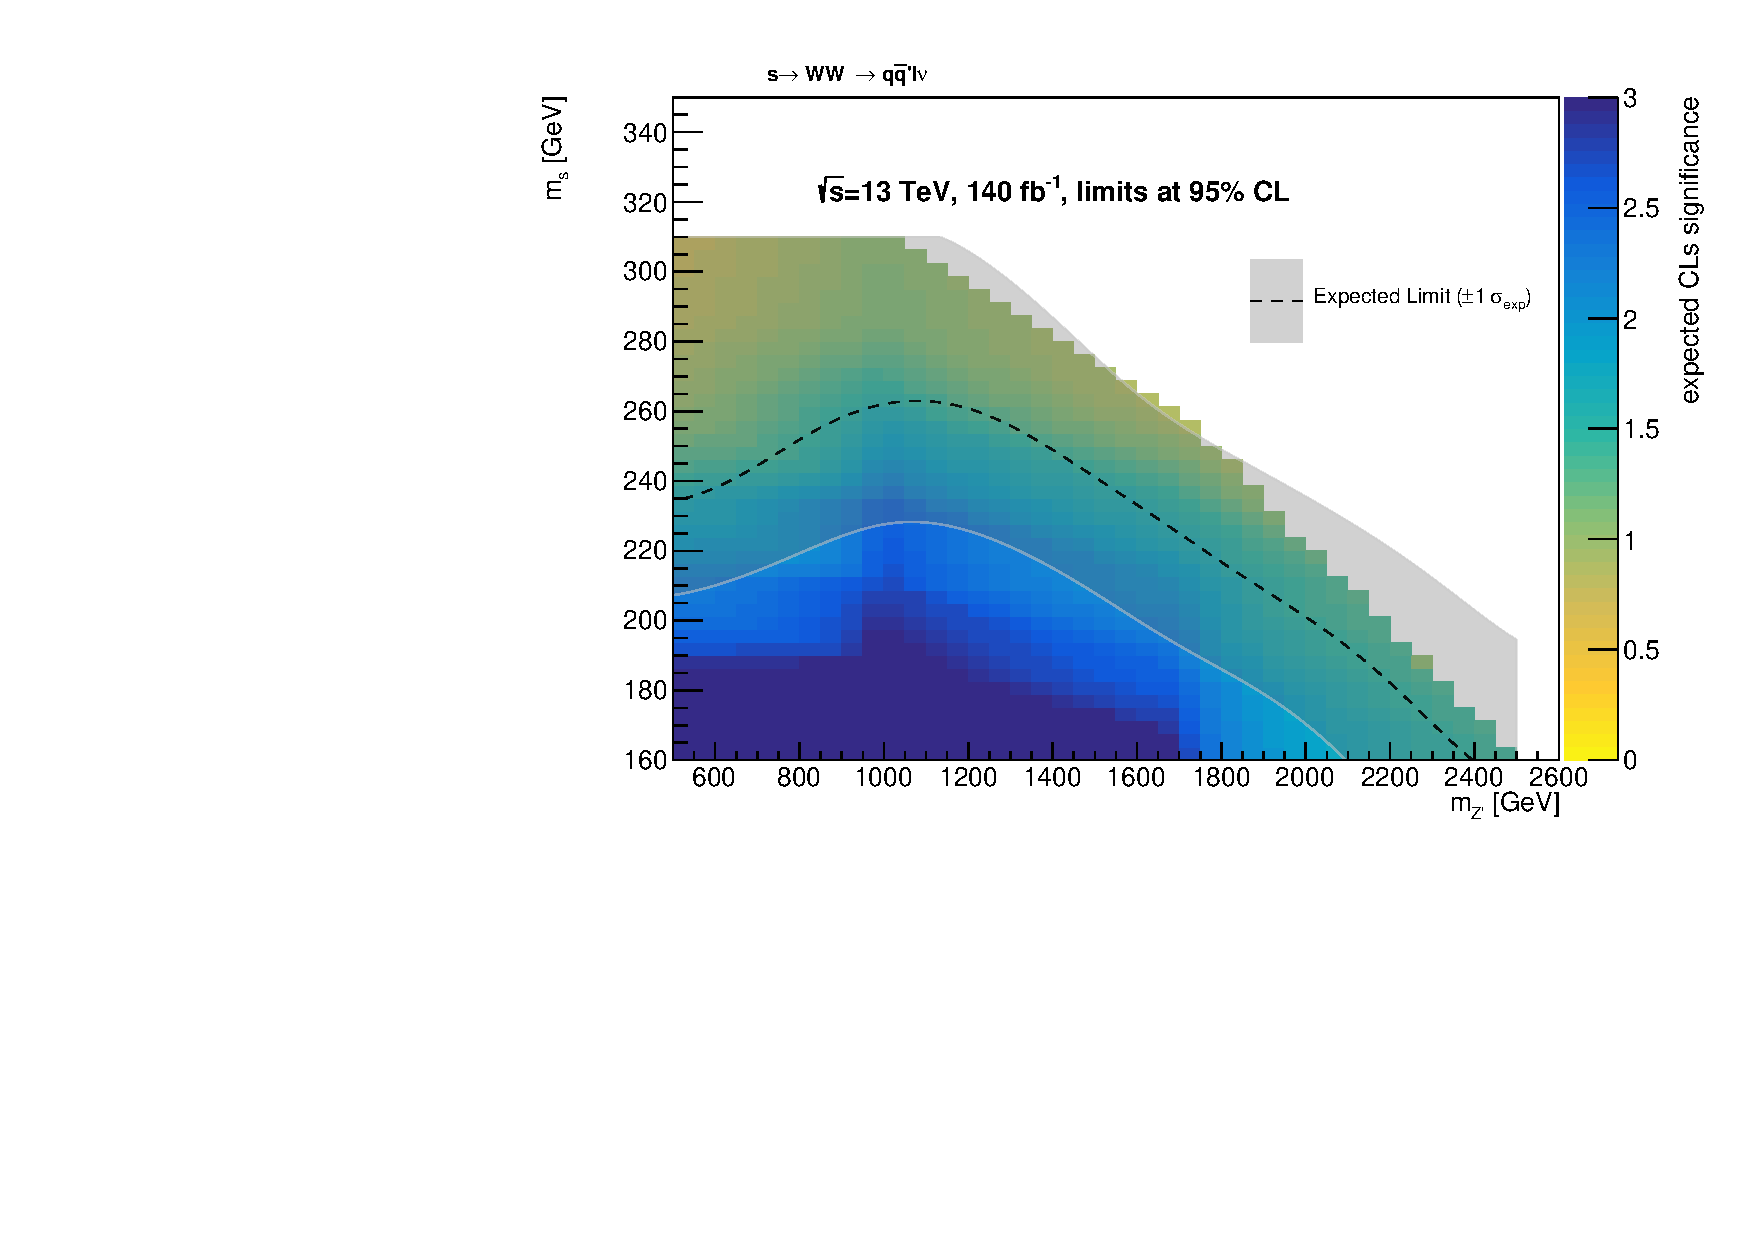
\includegraphics[width=\textwidth]{figures/exclude_combined_had_comparison_merged.pdf}
         \caption[]{Merged category}
         \label{fig:merged_sensitivity}
     \end{subfigure}
     \hfill
     \begin{subfigure}[b]{0.49\textwidth}
         \centering
         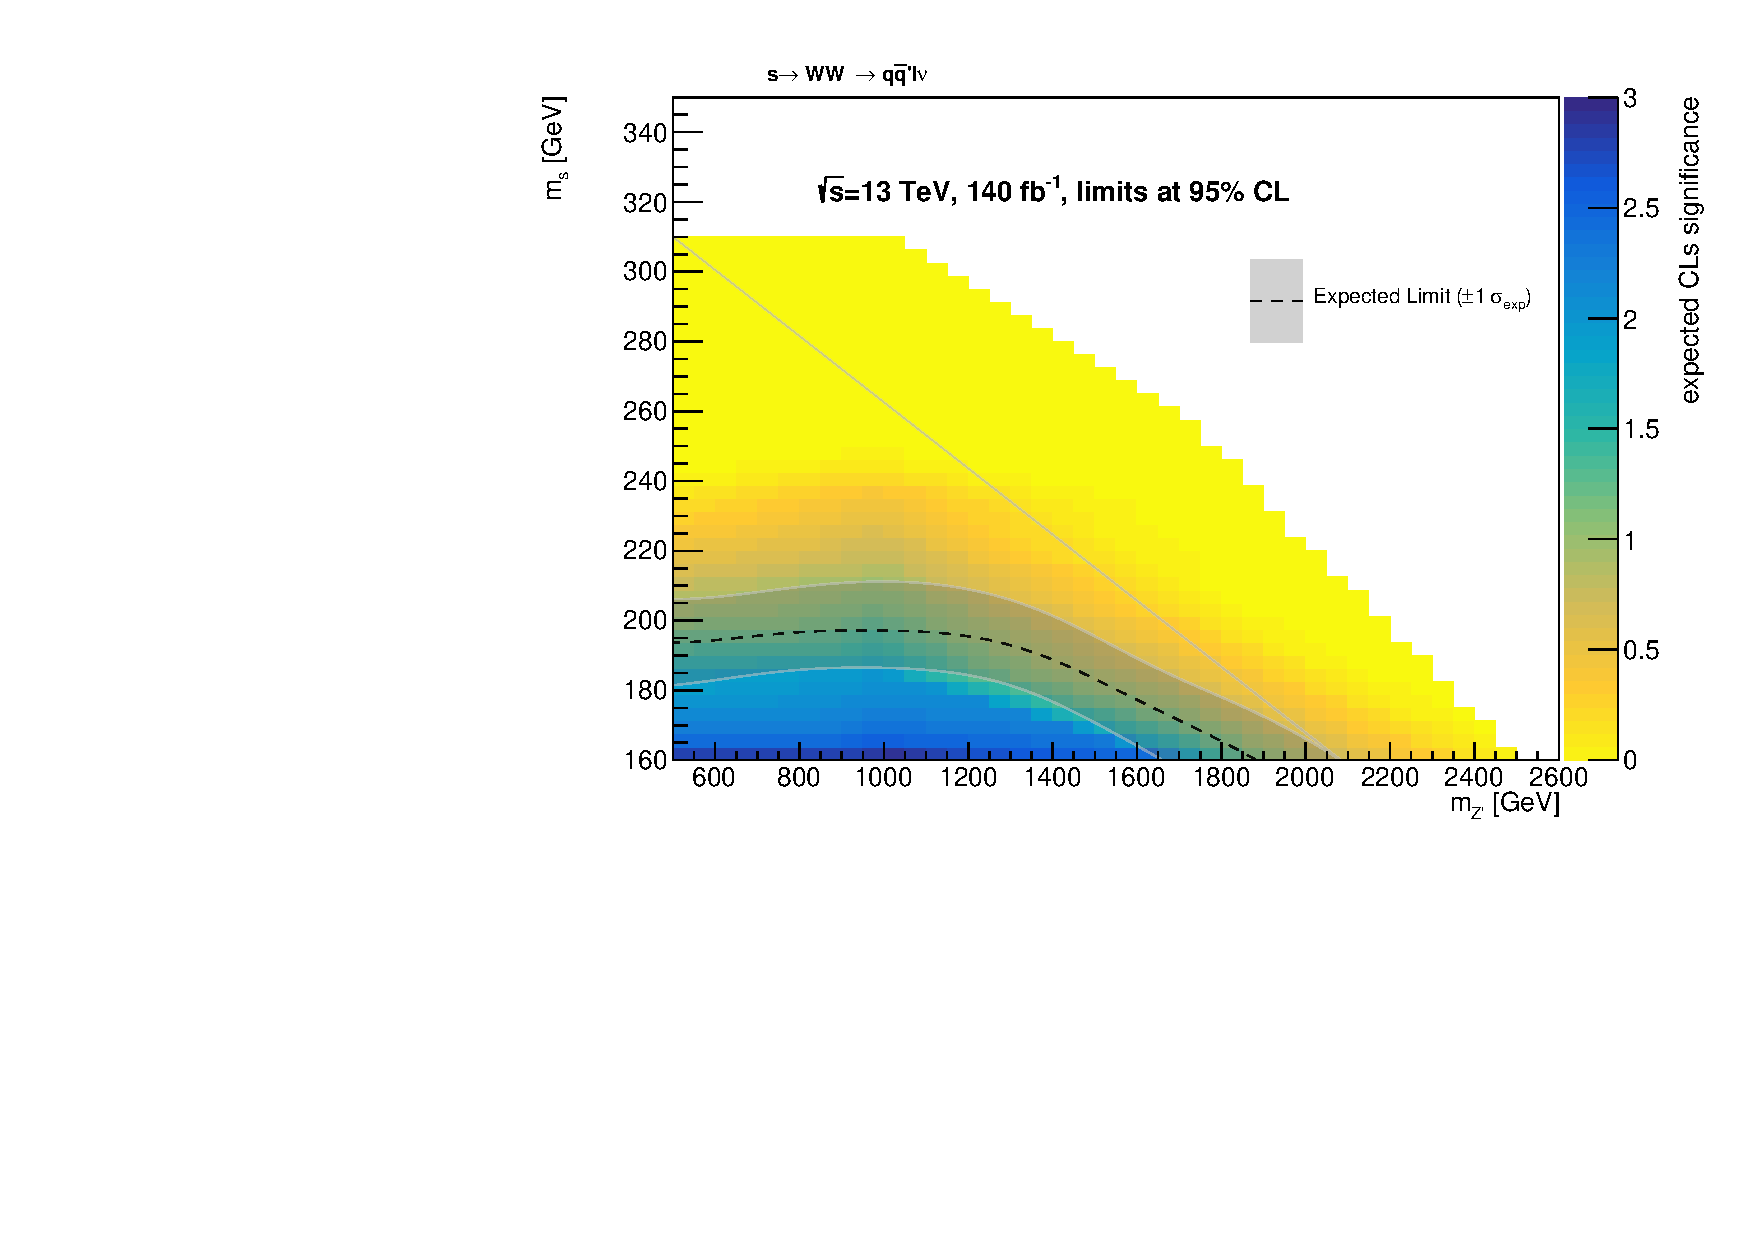
\includegraphics[width=\textwidth]{figures/exclude_combined_had_comparison_resolved.pdf}
         \caption[]{Resolved category}
         \label{fig:resolved_sensitivity}
     \end{subfigure}
\caption[]{CLs significance as a function of m$_\text{S}$ and m$_\text{Z'}$ within the individual categories}
\label{fig:sensitivity_categories}
\end{figure}

\subsubsection{Combined SR}

Figure \ref{fig:sensitivity_full} shows the sensitivity estimate for the combined merged+resolved SR, both with and without the signal grid interpolation and CLs contour. The significance grid on the left is designed to match the format in which the sensitiviy estimates are presented for the hadronic channel in figure \ref{fig:sensitivity} to allow for a more direct comparison. This preliminary comparison suggests that the semileptonic decay channel could offer comparable or even superior sensitivity compared with the hadronic channel. 

\begin{figure}[H]
     \centering
     \begin{subfigure}[b]{0.49\textwidth}
         \centering
         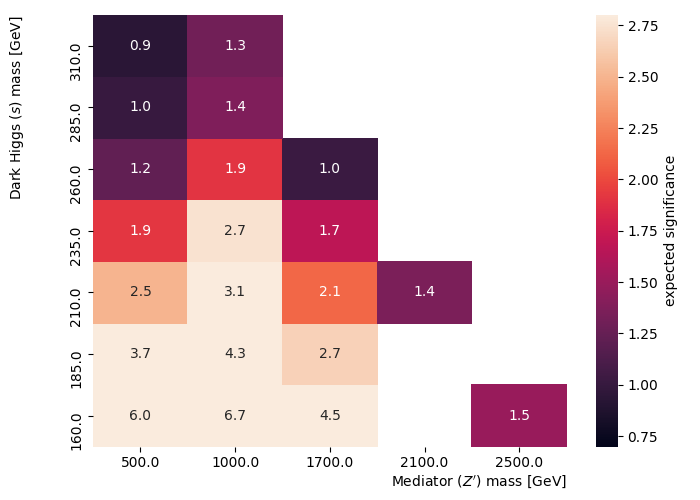
\includegraphics[width=\textwidth]{figures/semilep_sensitivity.png}
         \caption[]{Significance Grid}
         \label{fig:grid_sensitivity}
     \end{subfigure}
     \hfill
     \begin{subfigure}[b]{0.49\textwidth}
         \centering
         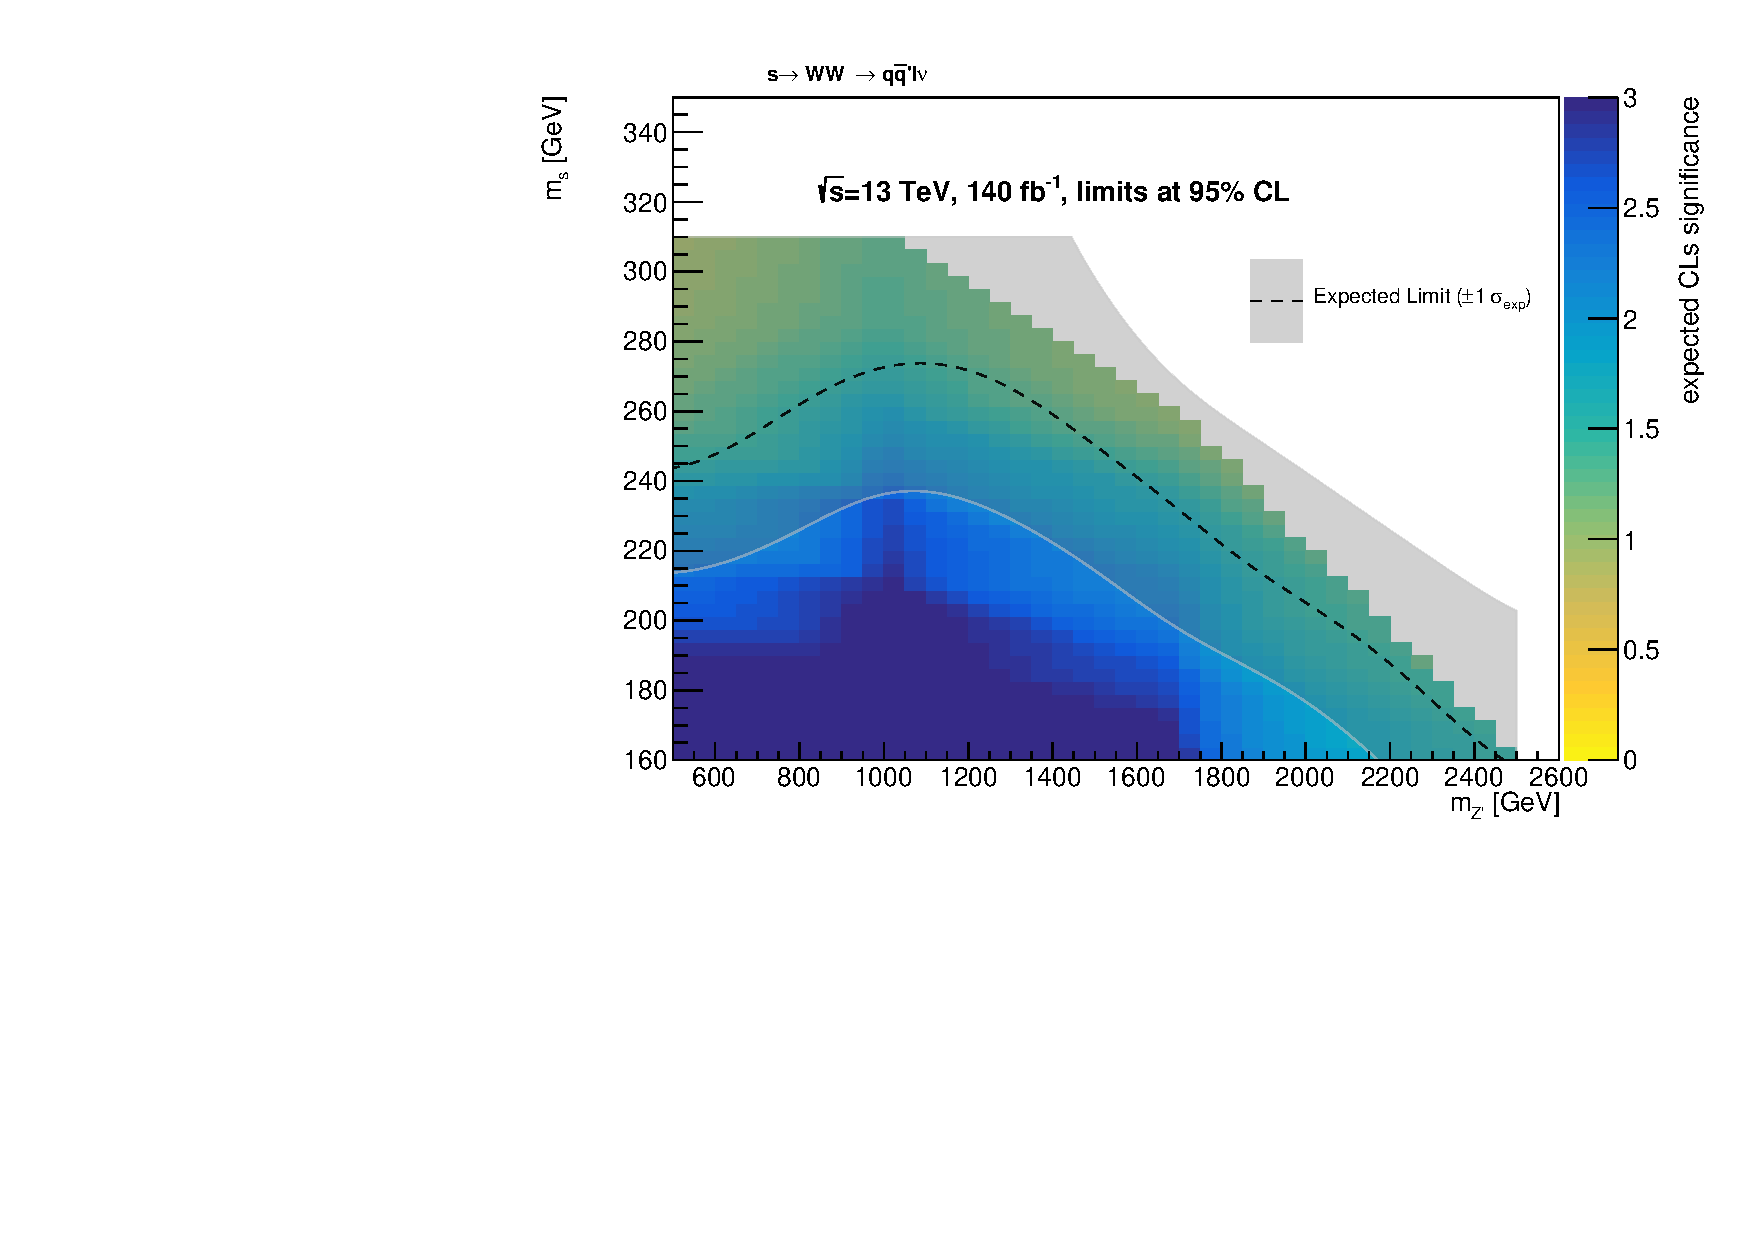
\includegraphics[width=\textwidth]{figures/exclude_combined_had_comparison.pdf}
         \caption[]{With interpolation and exclusion contour}
         \label{fig:interp_sensitivity}
     \end{subfigure}
\caption[]{CLs significances for the combined SR}
\label{fig:sensitivity_full}
\end{figure}

\section{Remaining Work and Outlook}

The analysis of the dark higgs signal model in the semileptonic WW decay channel continues to be developed and optimized. Preliminary sensitivity estimates suggest that this decay channel could offer valuable sensitivity to the model in addition to the hadronic channel currently nearing completion. The proposed thesis work will involve developing the analysis in the semileptonic channel in close collaboration with several colleagues here at UVic and at LMU in Munich. 

In addition to leading the UVic effort on this analysis, I share the role of ``analysis contact" with a colleague at LMU. The primary purpose of the analysis contact role is to liaise on behalf of the analysis group with conveners and other members of the wider analysis groups in ATLAS to which the analysis belongs. 

The major remaining tasks anticipated to complete the analysis are listed below in approximate order of priority. Table \ref{tab:timeline} summarizes the approximate timeline anticipated for completion of the remaining work, subsequent stages of approval within the ATLAS collaboration and publication of results. 
 
\subsection{Electron-Muon Differences}

The  algorithm presently applied to remove overlap between leptons and large-R jets appears to cause significant differences in jet reconstruction between semileptonic decays with a muon (i.e. `muon channel') vs. an electron (i.e. `electron channel') in the final state. This results in systematic differences in various large-R jet observables between the two channels, which cause substantially more events in the muon channel to pass the existing selections than in the electron channel. This asymmetry between the lepton and muon channels is both concerning from a physical perspective - events belonging to the lepton and muon channels should in principle produce statistically consistent distributions of observables with the exception of the observed lepton flavour - and it also reduces the statistics available to the analysis in the electron channel. 

Two approaches are being pursued to address these differences in large-R jet observables between the two lepton channels. 

The first approach is to move from the current ``LCTopo" jet reconstruction algorithm to track-assisted reclustered (TAR) jets \cite{TAR_jets}. This will allow for the implementation of a more sophisticated jet-lepton overlap removal algorithm currently being developed and studied by another physics analysis, which uses tracking information to remove tracks associated with the lepton, as well as any small-radius sub-jets overlapping with the lepton jet, then re-builds the TAR jet with the remaining small-radius sub-jets. 

The second approach is to split the electron and muon channels for cut optimization, and separately tune any cuts to which the two channels exhibit different responses. If this approach is taken in conjunction with the first approach, any lingering differences in TAR jet observables between the two channels with the improved overlap removal algorithm can be flexibly accommodated by tuning cuts associated with these observables separately to minimize any associated loss of signal statistics. 

\subsection{Signal Discrimination Variables}

Studies are ongoing to identify or develop variables which could offer useful discrimination between signal and background in the semileptonic SR. These include jet substructure variables to help distinguish large-R jets produced by a boosted $W\rightarrow qq$ decay from eg. the QCD quark pair production in the W+jets background, as well as approaches to computing a reconstructed dark higgs mass that account for the presence of neutrino-induced \met\!. Once these studies are complete, a set of selection variables will be chosen which exhibit the best discrimination between signal and background. The expected signal significances will be evaluated for various ranges of cut combinations on the chosen variables within each SR (eg. the merged category of the muon channel)  to determine the optimal cut placements. The expected signal significance is defined as \cite{cowandiscovery}:

\begin{equation}
  Z = \sqrt{2\left[
    \ln\left( \frac{(s+b)(b+\sigma_b^2)}{b^2 + (s+b)\sigma_b^2} \right)
    - \frac{b^2}{\sigma_b^2}\ln\left( 1 + \frac{\sigma_b^2 s}{b(b+\sigma_b^2)} \right)
  \right]}
  \label{eq:asimovsig}
\end{equation}
\noindent where $s$ is the expected number of signal events, $b$ is the expected number of background events and $\sigma_b$ is the statistical uncertainty on the expected number of background events.

\subsection{Optimize the W+jets and $\bm{t\bar{t}}$ CRs}

Once the signal selection is tuned and finalized, the CRs can be studied, and the effects of any cut reversals in addition to the basic definitions presented in Sections 6.2.3 and 6.2.4 can be studied to optimize the performance of the CRs. The performance of the CR is ultimately determined by its ability to isolate the background process of interest with sufficiently high statistics, low signal contamination and kinematic similarity to the SR to offer a reliable scaling factor for the background of interest in the SR. Data-MC comparisons with the CR-provided scaling factor can be studied in validation regions chosen explicitly to have kinematics similar to the SR to test the validity of the assumption that the scale factor determined in the CR is applicable to the SR. 

\subsection{Experimental and Modeling Systematics}

Once the SR and CR selections are optimized, experimental and modeling systematics will be added to the MC data in the form of associated variations on the nominal event weights, as described in Section 5.3. Many of the same systematics applied in the hadronic analysis and described in Sections 5.3.1 and 5.3.2 will likely be applied in the semileptonic channel, but the sizes and relative impacts of some systematics will differ. 

\subsection{Finalize the Fit with Full Systematics}

With the analysis regions finalized, the fit described in Section 7 will be updated with the final region definitions. The systematics will be added to the fit as uncertainties on the expectation value of their associated nuisance parameters in the likelihood function \cite{Baak:2014wma} used for the fit. 

\subsection{Unblinding and Publication}

When the analysis cuts are finalized and the fitting framework is in place, the analysts will request approval from the conveners of its ``Exotics" and ``JDM" (jets+DM) physics group and sub-group, respectively, to ``unblind" the SR. This means that rather than fitting to mock data generated to be statistically consistent with the MC in the SR, the fit will be performed with the actual ATLAS data in the SR to search for an above-background excess. If no excess is found, the observed CLs values can be used to set final exclusion limits based on the data.  

Following unblinding, the aim is to publish the results as an open-access article in a physics journal.

\begin{table}[H]
\centering
\caption{Tentative Timeline for Remaining Work}
\label{tab:timeline}
\begin{footnotesize}
\renewcommand{\arraystretch}{1.5}
\begin{tabular}{|p{30mm}|p{20mm}|p{100mm}|}
\hline
\textbf{Goal} & \textbf{Target Date} & \textbf{Discussion}  \\ \hline
Finalize variables and regions for selection & September 2020  & There is nothing blocking progress to this end, but time is required to develop and study new variables and finalize the choices of analysis regions within which to optimize.     \\ \hline
Finalize optimized SR and CR selections & November 2020      &   We are potentially dependent upon the timeline of ongoing work in another analysis towards developing an improved lepton-jet overlap removal (OR) algorithm using tracking information. While a preliminary version exists and has been implemented in our analysis code, final selection optimization cannot take place until the improved OR algorithm is implemented, if we wish to make use of it. The stated timeline for the improved algorithm is several months.  \\ \hline
Add experimental and modeling systematics to MC and fit  & December 2021s & We will likely be able to make use of most or all of the existing infrastructure in the code framework used by the hadronic channel for adding the systematic variations to the MC. However, the technical details of implementing them in the fit will differ due to the different fitting frameworks used by the two analyses.        \\ \hline
Request editorial board & January 2021  & A request is made for an editorial board (EB) when the analysis strategy is in place and documented in a supporting note. The EB is usually formed 1-1.5 weeks after a request is made.    \\ \hline
Request subgroup approval   & February 2021 &  A request for subgroup approval typically takes place $\sim$4 weeks after obtaining an EB.     \\ \hline
Unblind the SR  & April 2021 & Once the analysis is approved by the subgroup, the SR can be unblinded. It typically takes $\sim$9 weeks to obtain subgroup approval after it is requested, as modifications may need to be made to the analysis strategy in response to feedback received during the approval process.    \\ \hline
Request group approval of analysis and paper draft & June 2021 & Group approval is typically requested $\sim$7 weeks after the analysis obtains subgroup approval. The group approves both the analysis and the paper draft in one step.  \\ \hline
Circulate the paper draft to the ATLAS collaboration & August 2021 & It typically takes $\sim$6 weeks to receive group approval. Once received, the paper is circulated to the entire ATLAS collaboration for comment. \\ \hline
Publish results & Fall 2021 & The anticipated timeline for publication is very approximate, and may depend on the details of the results to be included.  \\ \hline
\end{tabular}
\end{footnotesize}
\end{table}

\bibliography{bibliography}
\bibliographystyle{unsrt}

\end{document}